\chapter{Results and Discussion}
\label{Ch:Result and Discussion}
\section{Q-Learning}

\subsection{Basic Model}
To build basic model, we used portfolio value change as a reward function, which means the agent will choose the action that will increase the expected portfolio value the most. We used two decimal of price change pair as a state.

We adjusted the parameters to give better performance. The learning rate($\alpha$), which decides the impact of new data on the existing Q-table, was set as 0.0001 based on experiment. The discount factor($\gamma$), which discounts the sum of future reward was set as 0.9. The epsilon($\epsilon$) was set as 0.9 and for every time period it is decreased 1\% until it reaches 0.01. It is in order to let the actions be chosen more randomly for exploration in the earlier times, since Q-table doesn’t contain much information. However later times’ actions are more likely to be chosen based on Q-table with smaller epsilon value. With those parameters, we trained the Q-table for each dataset 3000 episodes each.

As we trained on 10 training datasets, the performances of the basic model on each dataset didn’t have distinct patterns. Usually, the portfolio gains by the model were way better(3~4 times final portfolio value) than benchmark, but training results from 4th, 7th, 8th, 9th training set were similar or even below the benchmark gains. Each plot below has two subplots. The upper plot shows how the final portfolio value changes over every episode, and using the last episode’s data we drew bottom plot which shows the portfolio value change over days. Compared to those of training 1 with KLAC and SKX data and training 10 with NVDA and SKX data, the results of training 4 and training 9 are not good. We didn’t find any clear reason behind this. The dimension of Q-table is steadily increased with more training as shown in below plot.

\begin{figure}[H]
\begin{subfigure}{.5\textwidth}%
\centering
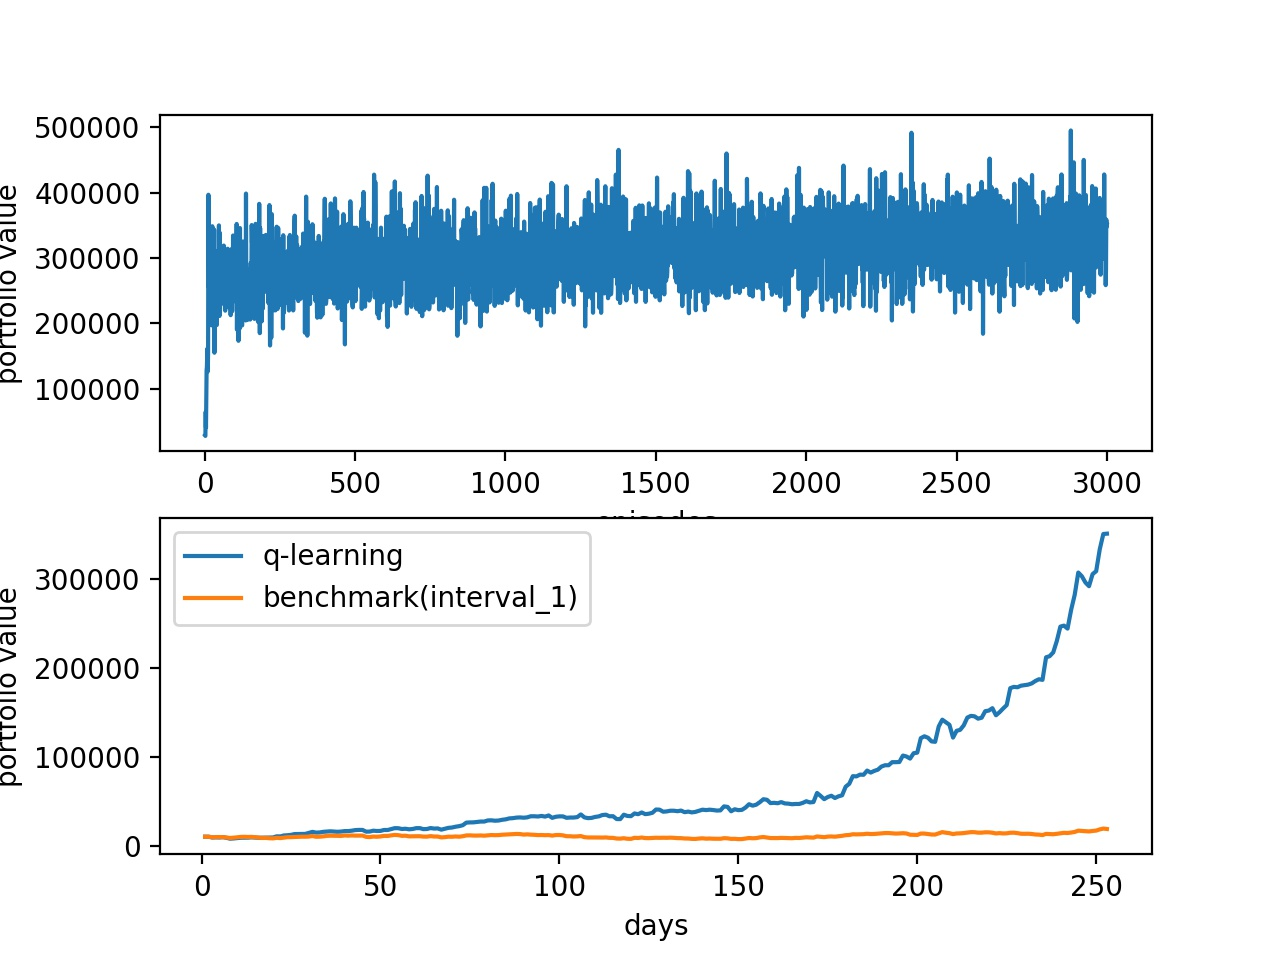
\includegraphics[clip, width=1.1\textwidth]{Graphics/q_learning_KS1.eps} \caption{Training 1 (KLAC \& SKX)} 
\end{subfigure}%
\begin{subfigure}{.5\textwidth}%
\centering
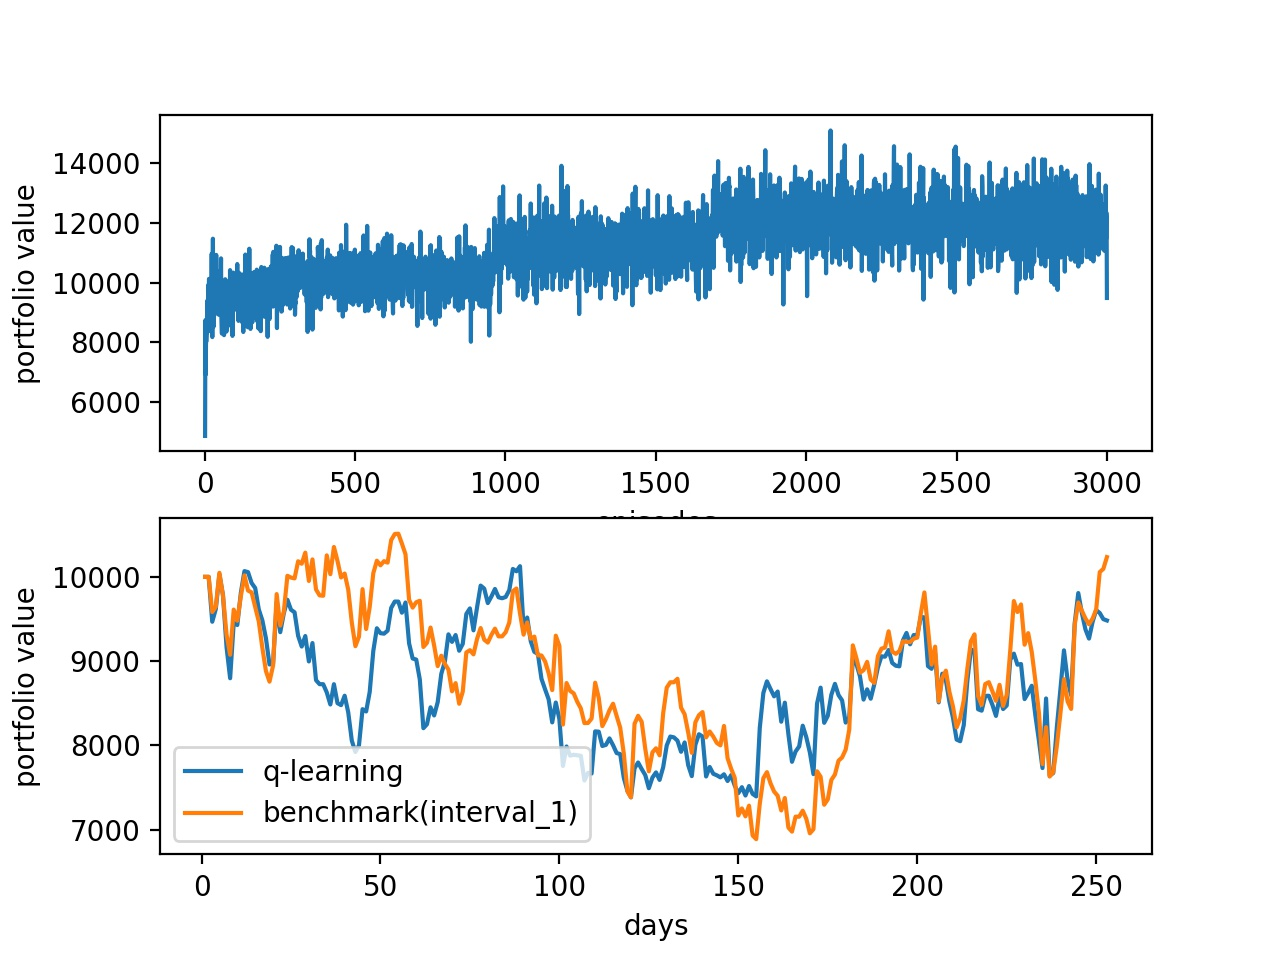
\includegraphics[clip, width=1.1\textwidth]{Graphics/q_learning_AM4.jpg} \caption{Training 4 (AMD \& MTN)}
\end{subfigure}%
\vspace{0.1cm}
\begin{subfigure}{.5\textwidth}%
\centering
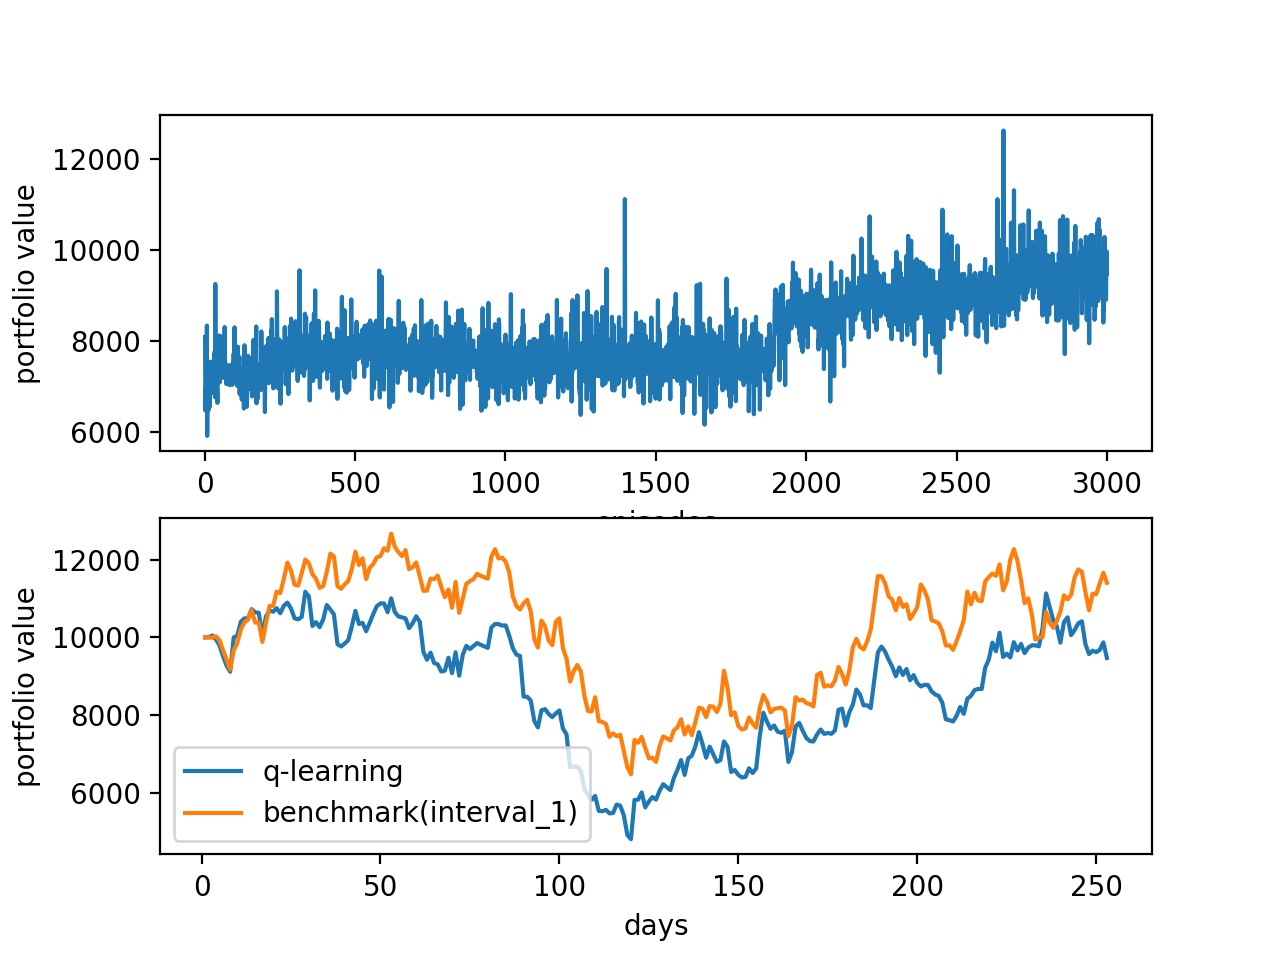
\includegraphics[clip, width=1.1\textwidth]{Graphics/q_learning_MP9.jpg} \caption{Training 9 (MU \& PPC)}
\end{subfigure}%
\begin{subfigure}{.5\textwidth}
\centering
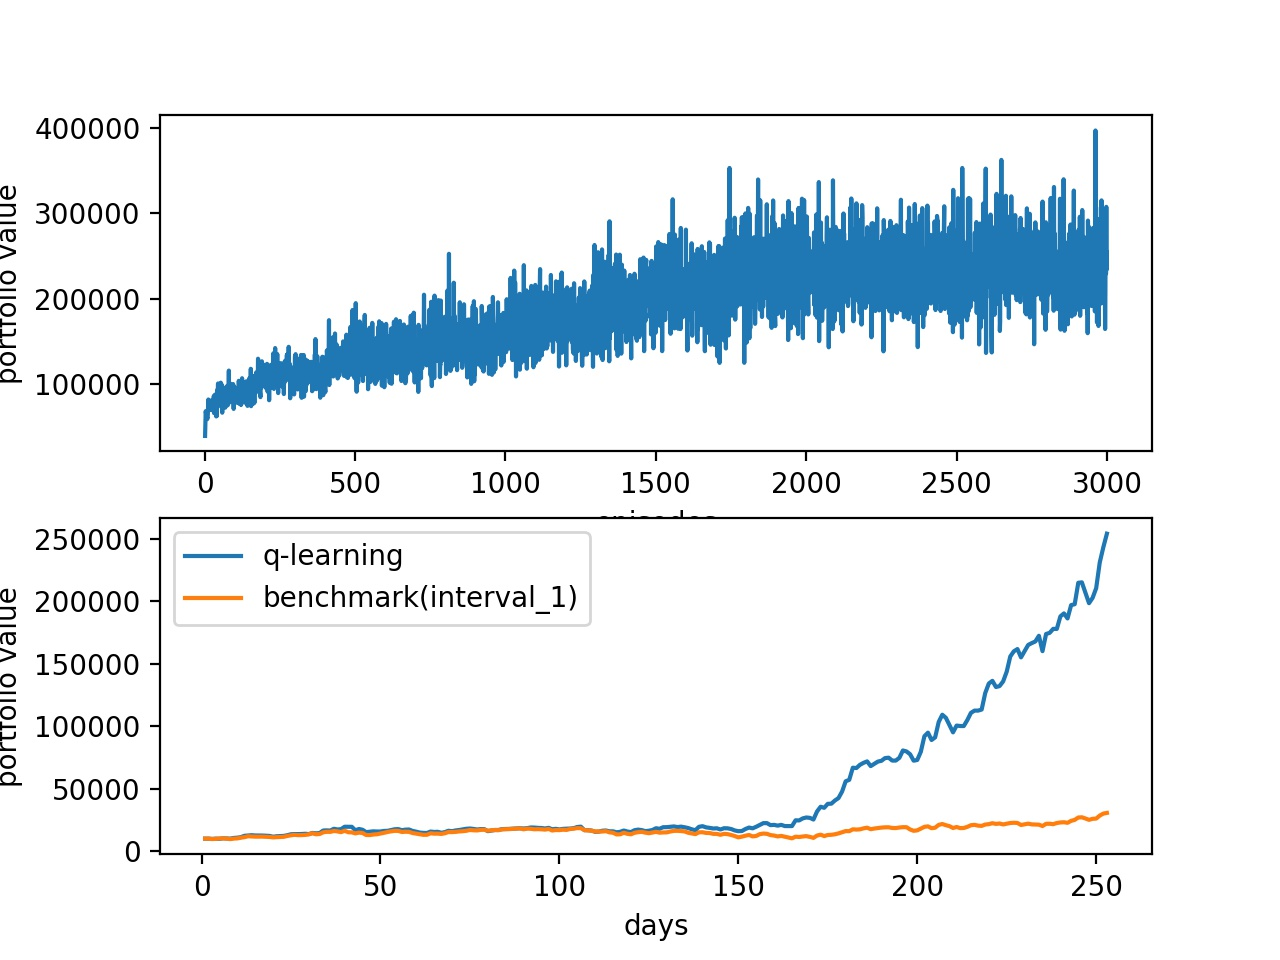
\includegraphics[clip, width=1.1\textwidth]{Graphics/q_learning_NS10.jpg} \caption{Training 10 (NVDA \& SKX)}
\end{subfigure}%
\vspace{0.1cm}
\begin{figure}
\begin{center}
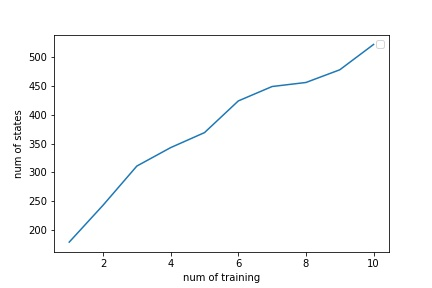
\includegraphics[clip, width=0.8\textwidth]{Graphics/dimension.jpg} \caption{Dimension change over training}
\end{center}
\end{figure}
\end{figure}%

Using the $Q$-table we trained, we tested on two test datasets(AMAT \& CAJ, FCX \& CAJ). Test results using FCX \& CAJ dataset usually showed better results. However more training didn’t guarantee better test results. For AMAT \& CAJ, the best test result was using the Q-table trained with 1 dataset, and further training tables made the test results’ portfolio value be decreased. On the other hand, for FCX \& CAJ, the best test result was with 8 times training Q-table, and before and after that the final portfolio value is below benchmarks. To check the reason why test results keep changing, we analyzed the actions taken in each result. Even the actions taken in the test using 9 times training, and using 10 times training differed a lot. The last plot which has 3 subplots is drawn using the FCX \& CAJ data. The first subplot is comparing the actions taken with 5 and 8 times training, while the second is comparing 8 times and 10 times, and the last is comparing 10 times and 9 times.
\vspace{0.05cm}
\begin{figure}[H]
\begin{figure}[H]
\begin{center}
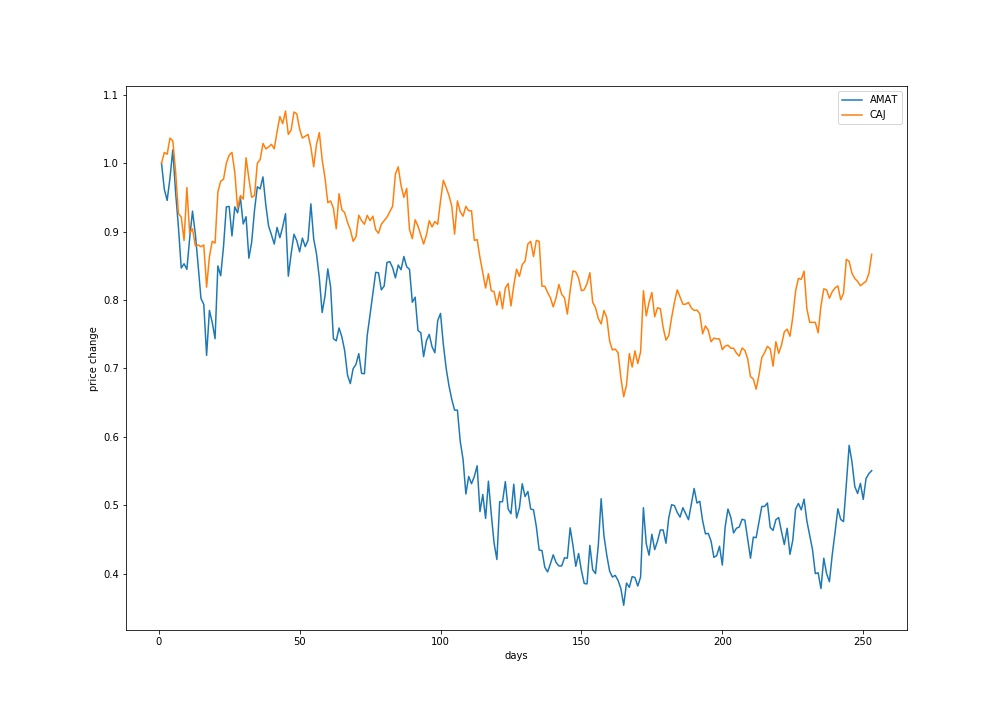
\includegraphics[clip, width=0.7\textwidth]{Graphics/test1_pricechange.jpg} \caption{TEST SET1 (AMAT \& CAJ) :PRICE CHANGE}
\end{center}
\end{figure}
\vspace{0.1cm}
\begin{subfigure}{.5\textwidth}%
\centering
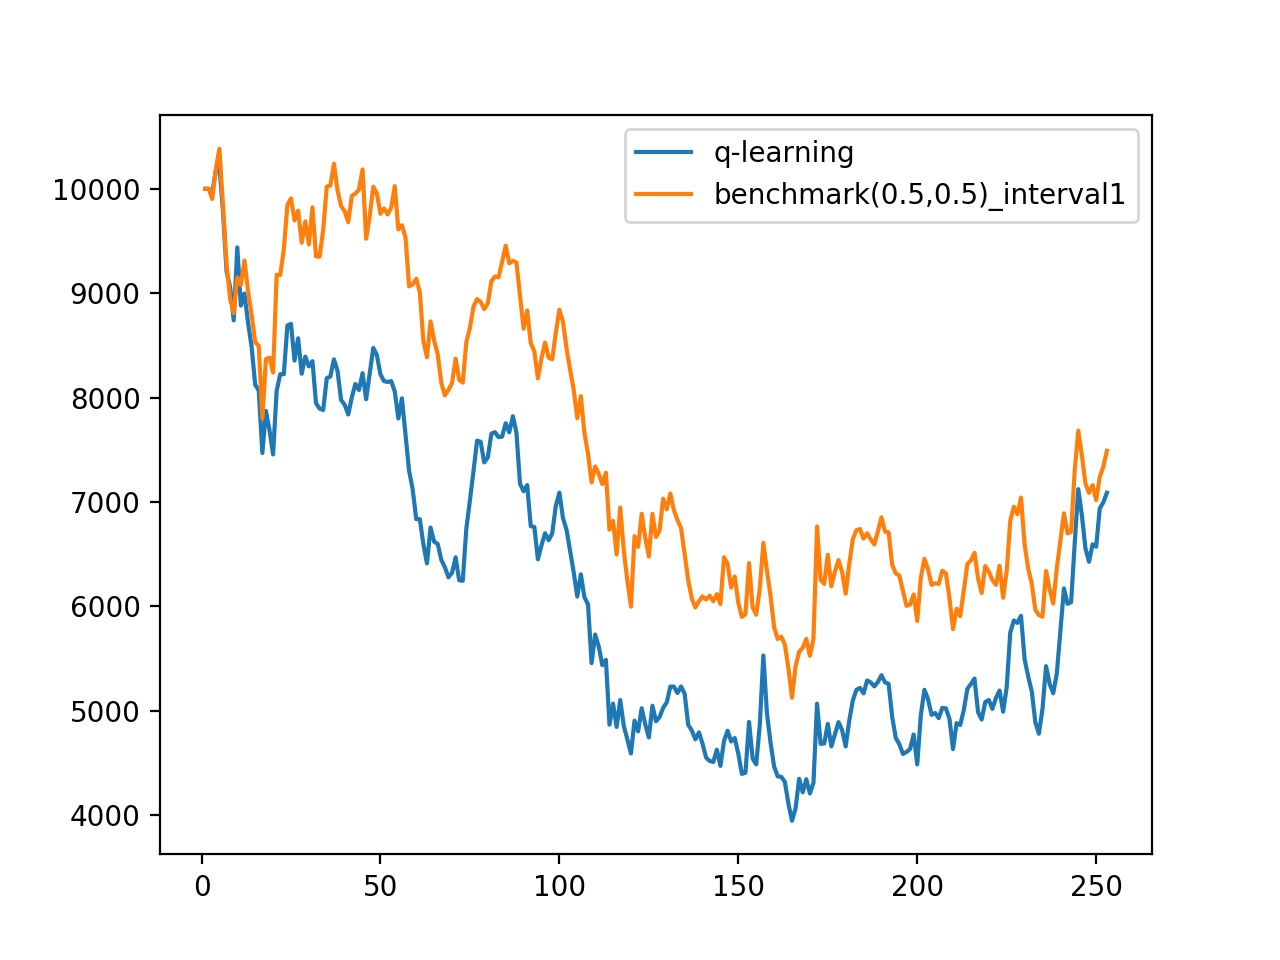
\includegraphics[clip, width=1.1\textwidth]{Graphics/test_KS1_AC_action.jpg} \caption{TEST SET1 (AMAT \& CAJ):1 training} 
\end{subfigure}%
\vspace{0.1cm}
\begin{subfigure}{.5\textwidth}%
\centering
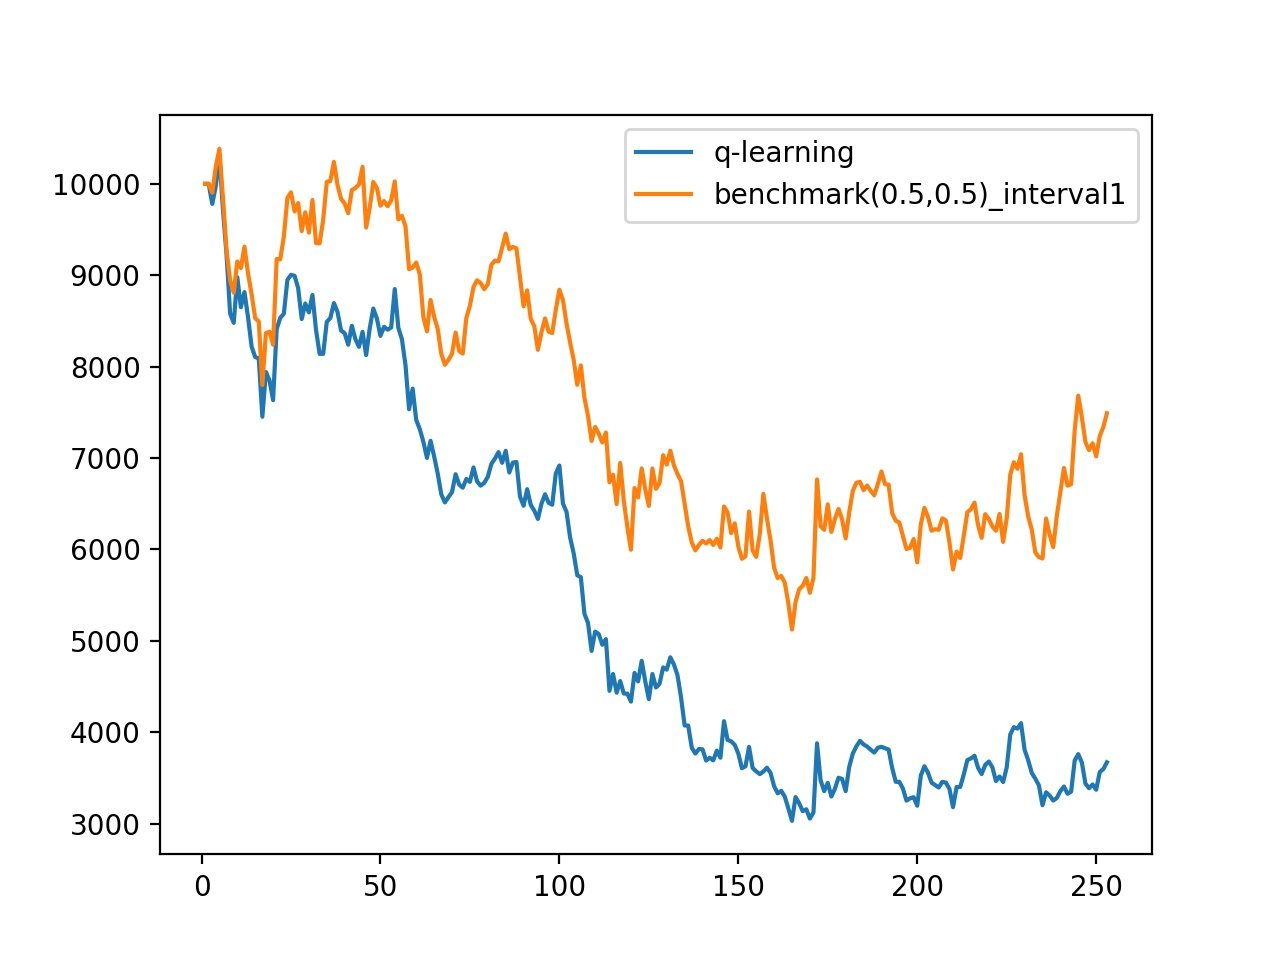
\includegraphics[clip, width=1.1\textwidth]{Graphics/test_LP3_AC_action.jpg} \caption{TEST SET1 (AMAT \& CAJ):3 training}
\end{subfigure}%
\end{figure}%

\newpage

\begin{figure}[H]
\begin{figure}[H]
\begin{center}
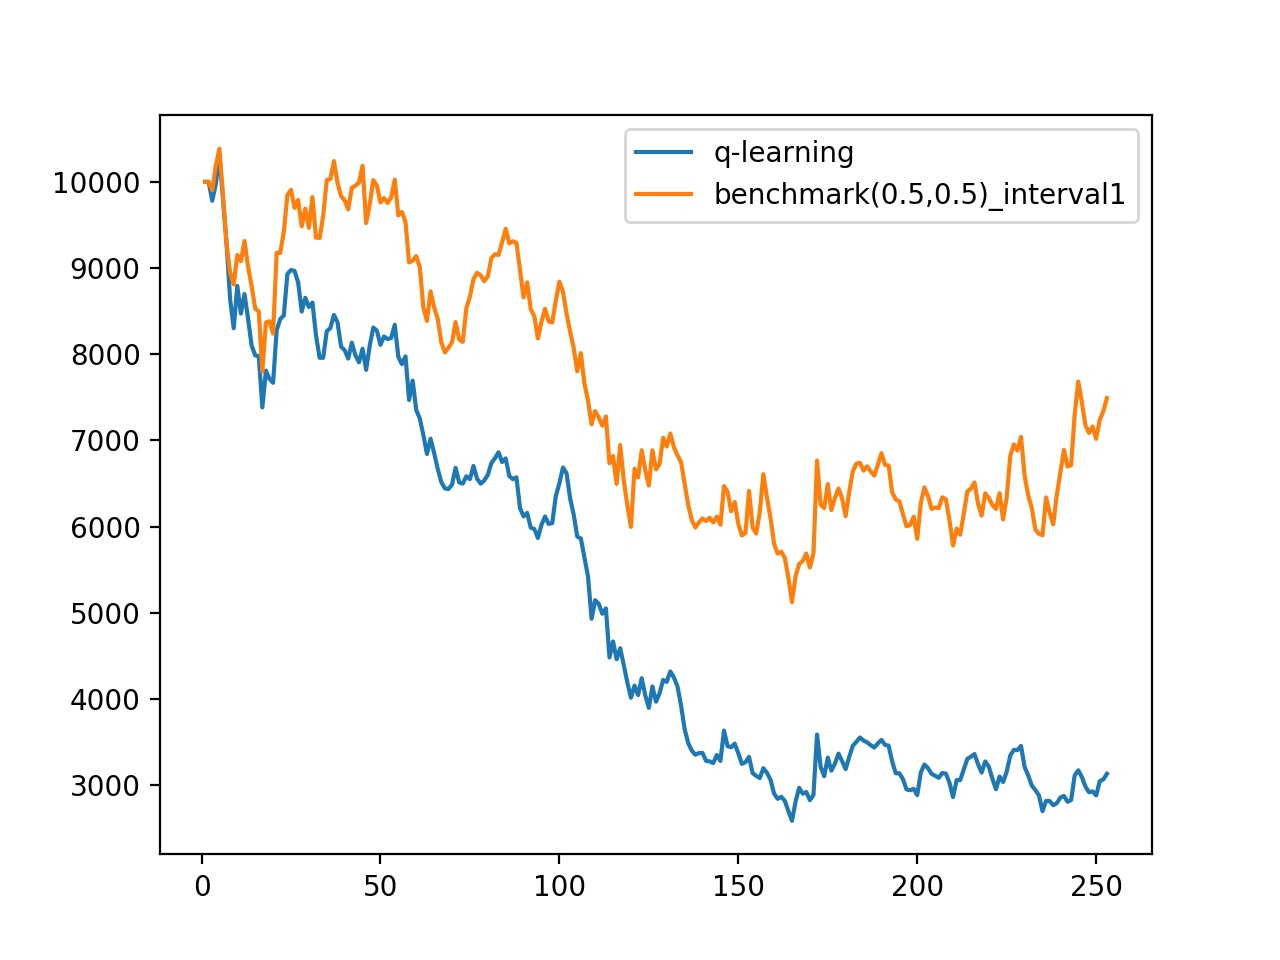
\includegraphics[clip, width=0.9\textwidth]{Graphics/test_NS10_AC_action.jpg} \caption{TEST SET1 (AMAT \& CAJ) : result with 10 training Q-table}
\end{center}
\end{figure}
\vspace{0.1cm}
\begin{figure}[H]
\begin{center}
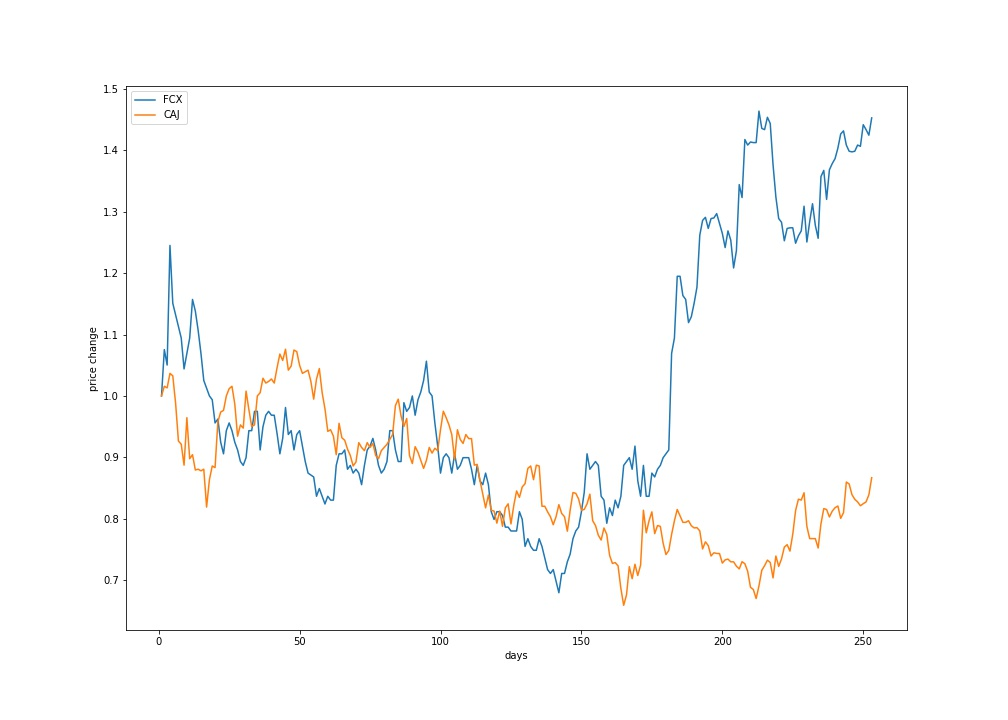
\includegraphics[clip, width=0.9\textwidth]{Graphics/test2_pricechange.jpg} \caption{TEST SET2 (FCX \& CAJ) : PRICE CHANGE}
\end{center}
\end{figure}
\vspace{0.1cm}
\end{figure}

\newpage

\begin{figure}[H]
\begin{subfigure}{.5\textwidth}%
\centering
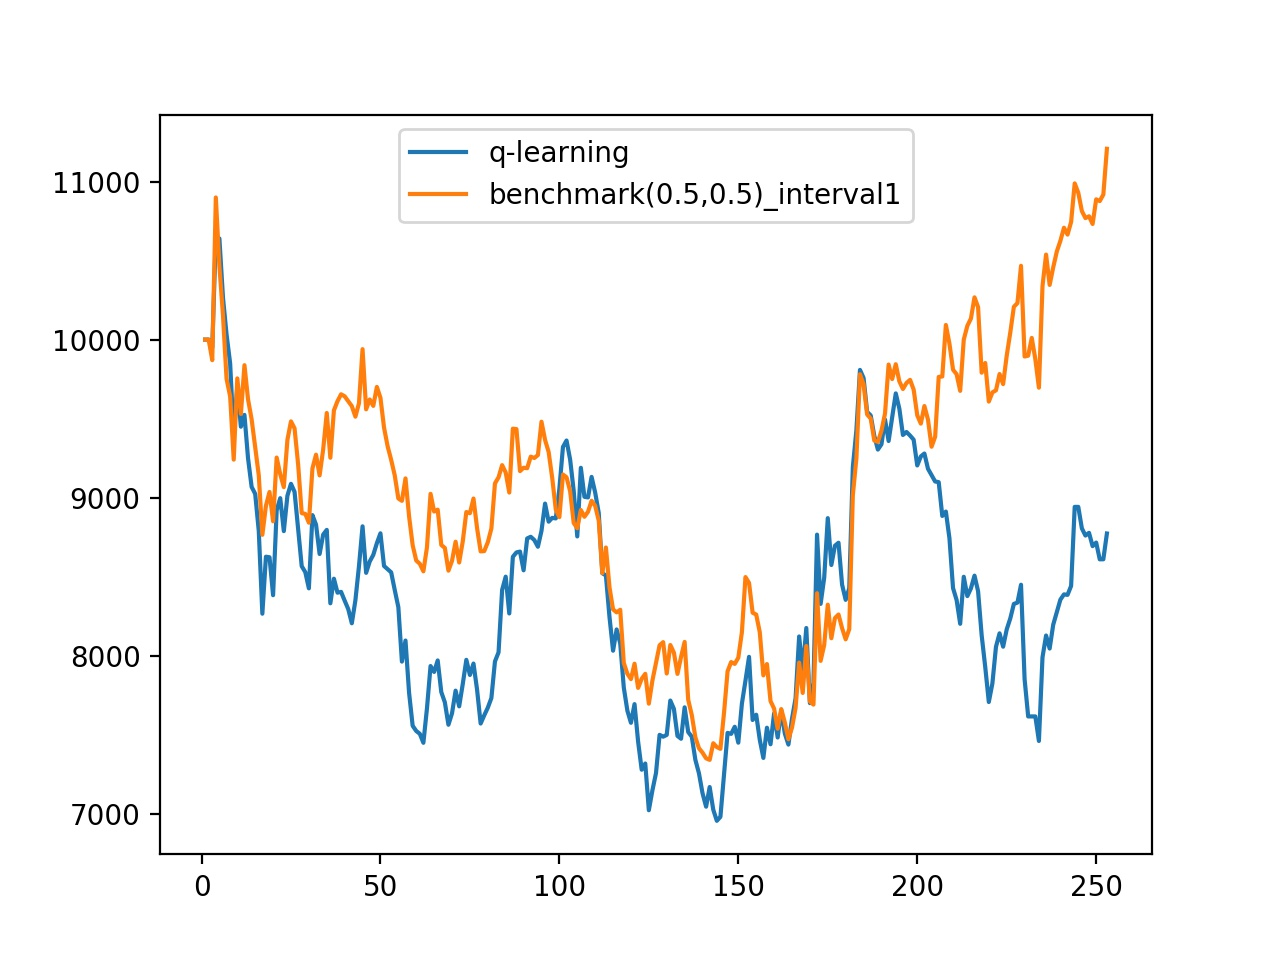
\includegraphics[clip, width=0.9\textwidth]{Graphics/test_NM5_FC_action.jpg} \caption{TEST SET2 (FCX \& CAJ): 5 training} 
\end{subfigure}%
\vspace{0.1cm}
\begin{subfigure}{.5\textwidth}%
\centering
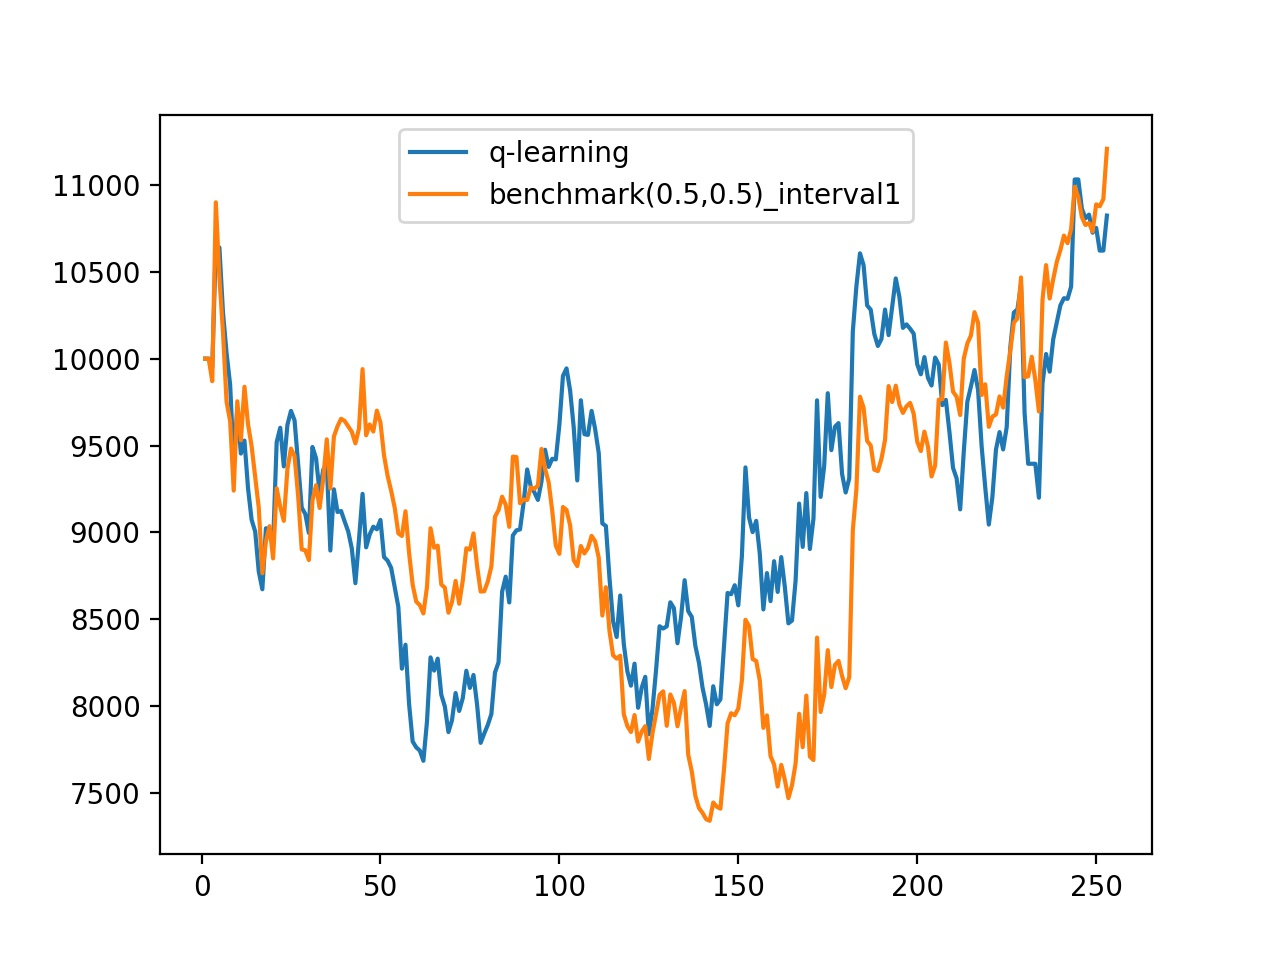
\includegraphics[clip, width=0.9\textwidth]{Graphics/test_AS8_FC_action.jpg} \caption{TEST SET2 (FCX \& CAJ): 8 training}
\end{subfigure}%
\begin{figure}[H]
\begin{center}
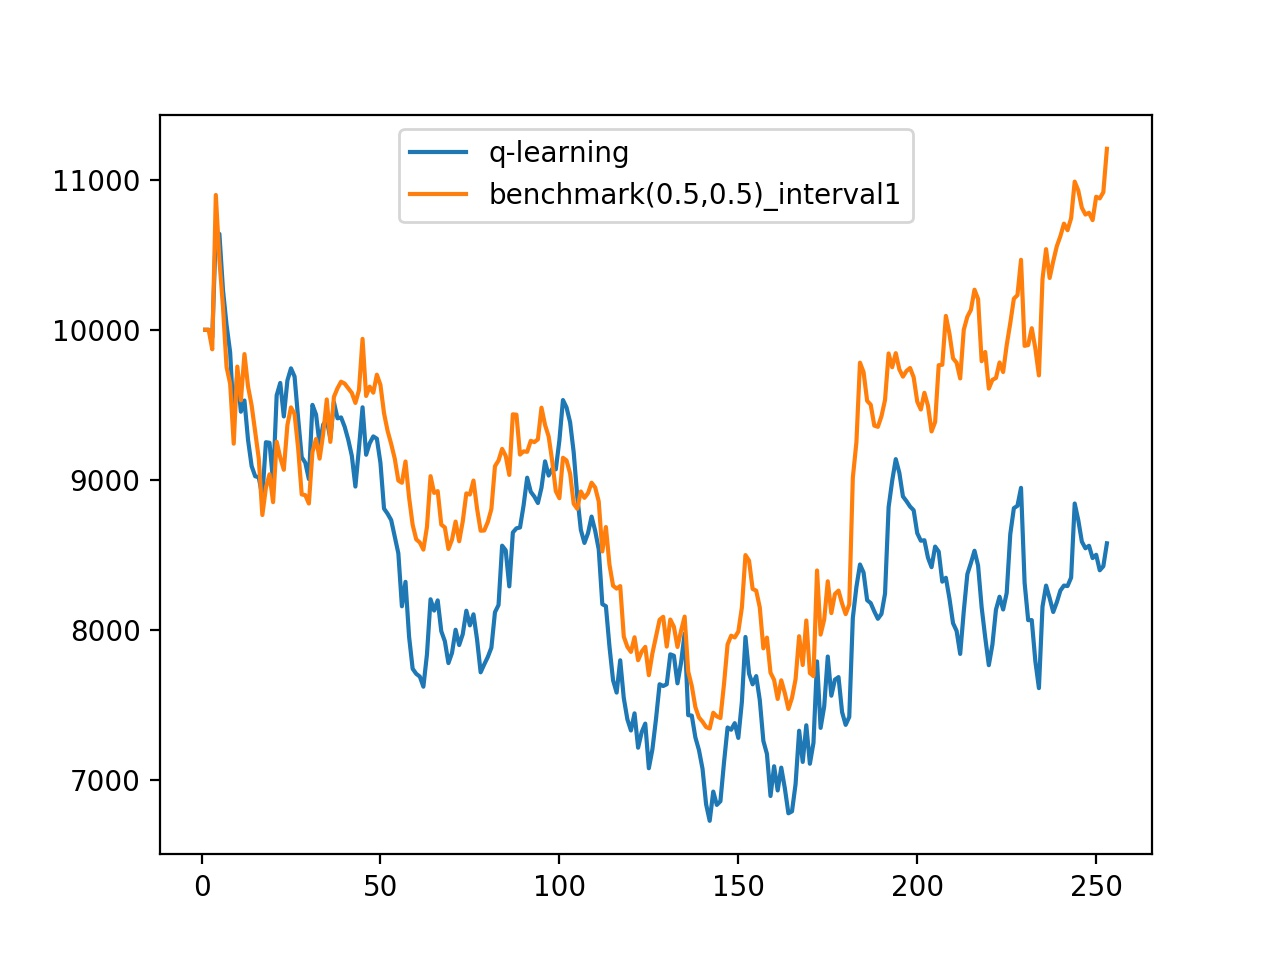
\includegraphics[clip, width=0.6\textwidth]{Graphics/test_NS10_FC_action.jpg} \caption{TEST SET2 (FCX \& CAJ) : result with 10 training Q-table}
\end{center}
\end{figure}
\begin{figure}[H]
\begin{center}
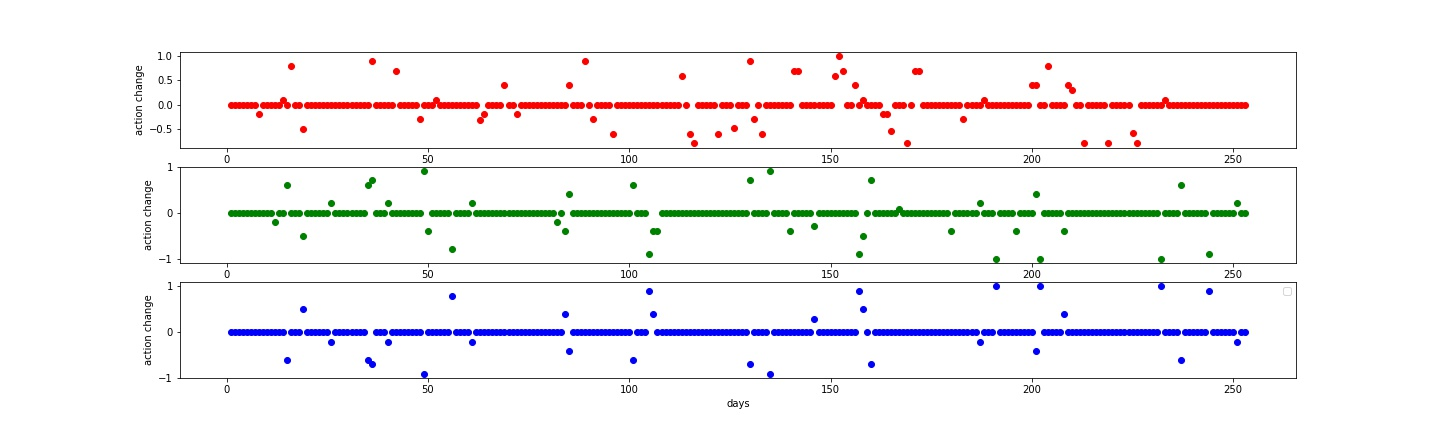
\includegraphics[clip, width=0.7\textwidth]{Graphics/actionchange3.jpg} \caption{ACTION CHANGE : (8 vs 5, 8 vs 10, 10 vs 9)}
\end{center}
\end{figure}
\end{figure}

\subsection{Linear Regression}
As for portfolio management, we should not only consider the  profit, but also the risk, thus we use the sharpe ratio $R=\frac{E(Rp)-Rf}{\sigma Rp}$ as reward function, where $E(Rp)$ is the expected portfolio return , $Rf$ is the risk free rate, and $\sigma Rp$ is the portfolio standard deviation. In our model, we let $Rf=0$, and $Rf=\frac{pv_t-pv_{t-1}}{pv_{t-1}}$. We use the pairs of two stocks’ simple linear regression functions’ slope as states $(a_n,k_n)$, and to generalize the states, we only keep one decimal of the slope.

\vspace{0.5cm}

\textbf{Using 10 pairs’s stocks’ one year data to train the} model
\begin{figure}[H]
\begin{subfigure}{.5\textwidth}%
\centering
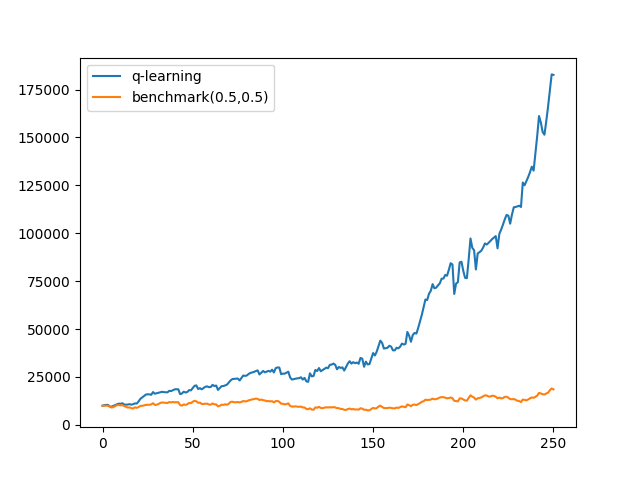
\includegraphics[clip, width=0.9\textwidth]{Graphics/trainParameterWithT.png} \caption{TRAIN 1 (KLAC \& SKX)
} 
\end{subfigure}%
\begin{subfigure}{.5\textwidth}%
\centering
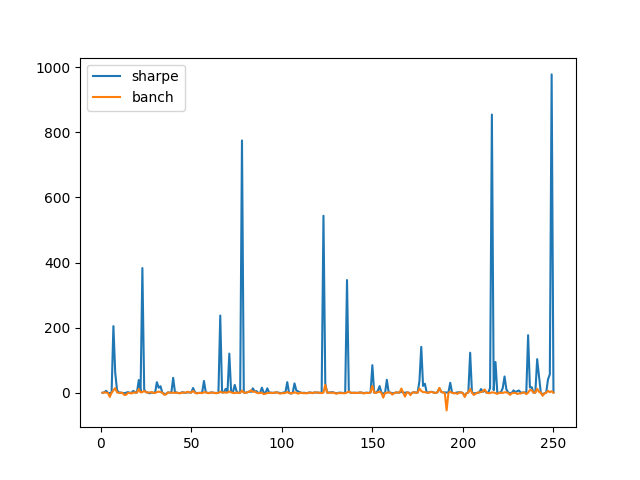
\includegraphics[clip, width=0.9\textwidth]{Graphics/trainParameterWTSharpe.png} \caption{Sharpe Ratio of TRAIN 1}
\end{subfigure}%
\vspace{0.1cm}
\begin{subfigure}{.5\textwidth}%
\centering
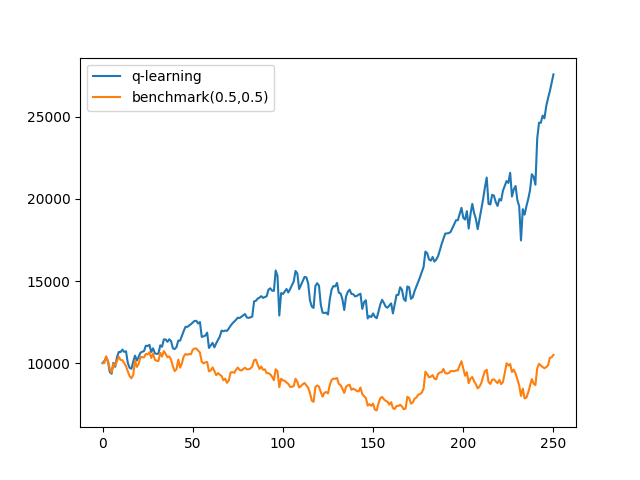
\includegraphics[clip, width=0.9\textwidth]{Graphics/trainParameter3WT.png} \caption{TRAIN 4 (AMD \& MTN))} 
\end{subfigure}%
\begin{subfigure}{.5\textwidth}%
\centering
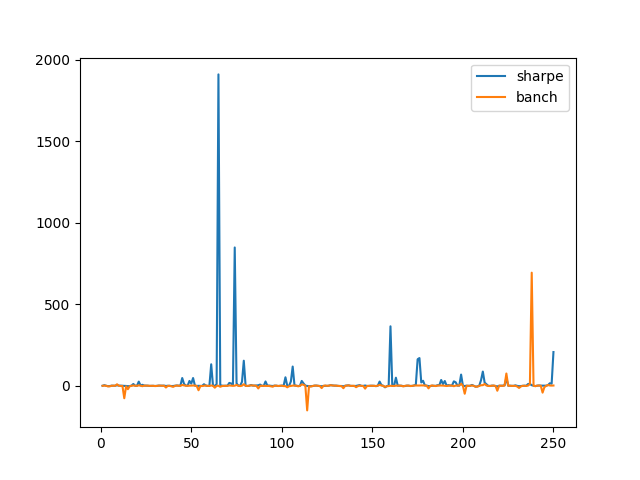
\includegraphics[clip, width=0.9\textwidth]{Graphics/trainParameter3WTS.png} \caption{Sharpe Ratio of TRAIN 4}
\end{subfigure}%
\vspace{0.1cm}
\begin{subfigure}{.5\textwidth}%
\centering
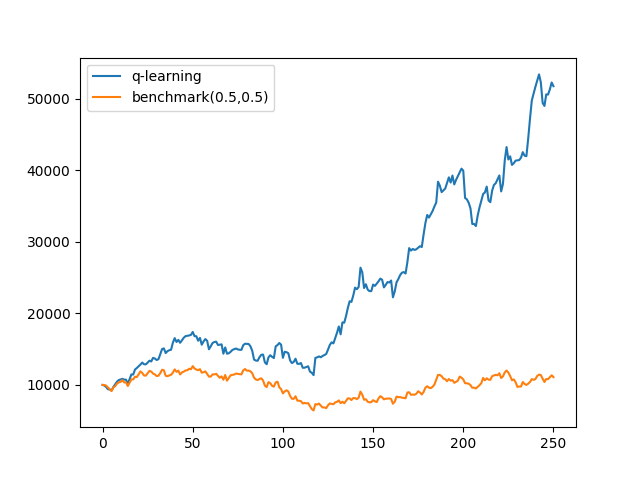
\includegraphics[clip, width=0.9\textwidth]{Graphics/trainPA9.png} \caption{TRAIN 9 (MU \& PPC))} 
\end{subfigure}%
\begin{subfigure}{.5\textwidth}%
\centering
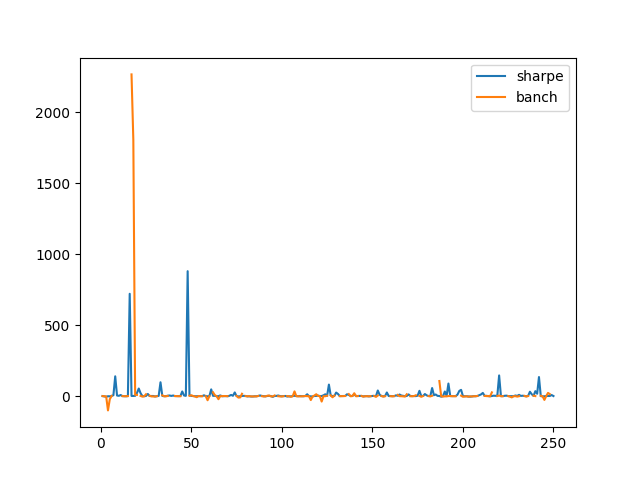
\includegraphics[clip, width=0.9\textwidth]{Graphics/trainPA9S.png} \caption{Sharpe Ratio of TRAIN 9}
\end{subfigure}%
\end{figure}

\newpage
Then we get the test result as follow:

\begin{figure}[H]
\begin{subfigure}{.5\textwidth}%
\centering
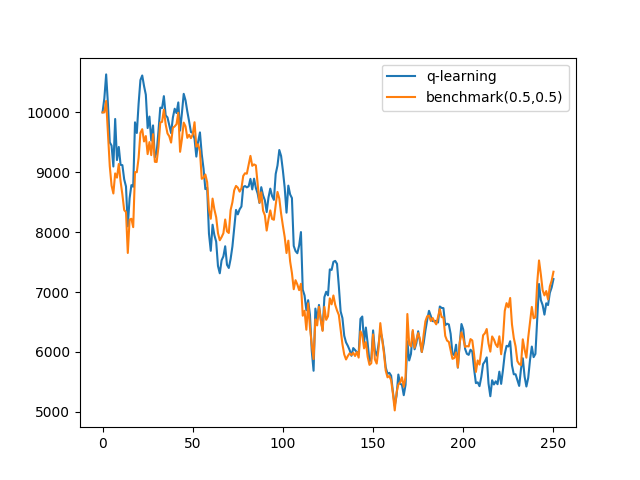
\includegraphics[clip, width=0.9\textwidth]{Graphics/TestAC3.png} \caption{TEST 1 (AMAT \& CAJ)} 
\end{subfigure}%
\begin{subfigure}{.5\textwidth}%
\centering
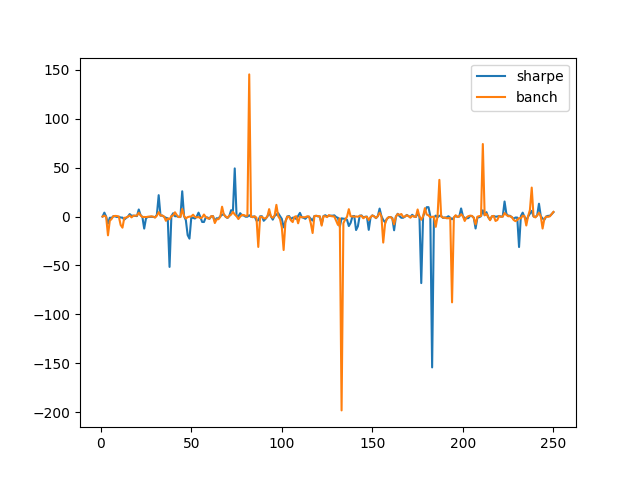
\includegraphics[clip, width=0.9\textwidth]{Graphics/TESTAC3S.png} \caption{Sharpe Ratio of TEST 1}
\end{subfigure}%
\vspace{0.1cm}
\begin{subfigure}{.5\textwidth}%
\centering
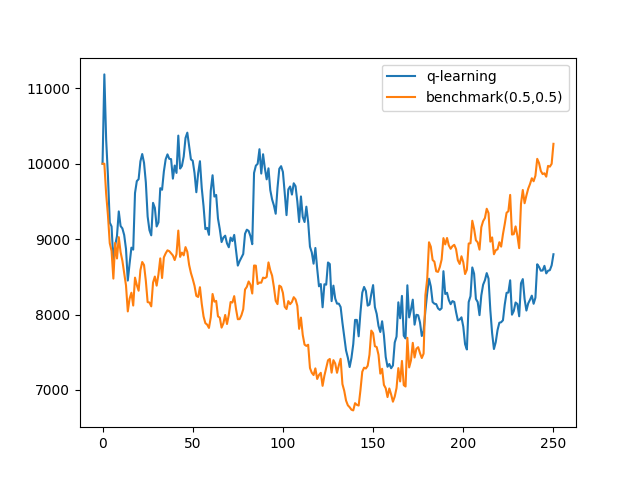
\includegraphics[clip, width=0.9\textwidth]{Graphics/TESTFC3.png} \caption{TEST 2 (FCX \& CAJ))} 
\end{subfigure}%
\begin{subfigure}{.5\textwidth}%
\centering
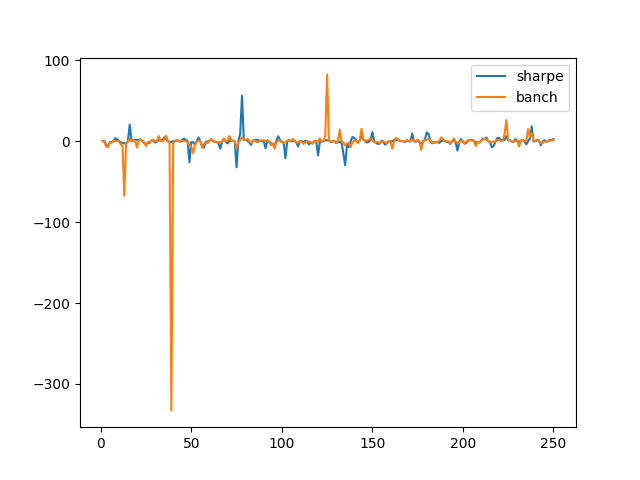
\includegraphics[clip, width=0.9\textwidth]{Graphics/TESTFC3S.png} \caption{Sharpe Ratio of TEST 2}
\end{subfigure}%
\vspace{0.7cm}
We are thinking that whether more days of a period can have a better result, so we use each 10 days as a period to get the regression functions.
\vspace{0.7cm}
\begin{subfigure}{.5\textwidth}%
\centering
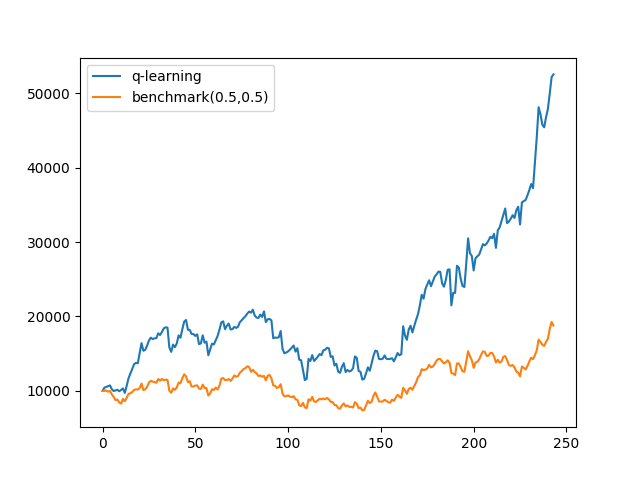
\includegraphics[clip, width=0.9\textwidth]{Graphics/trainPA00WT.png} \caption{TRAIN 1 (KLAC \& SKX)} 
\end{subfigure}%
\begin{subfigure}{.5\textwidth}%
\centering
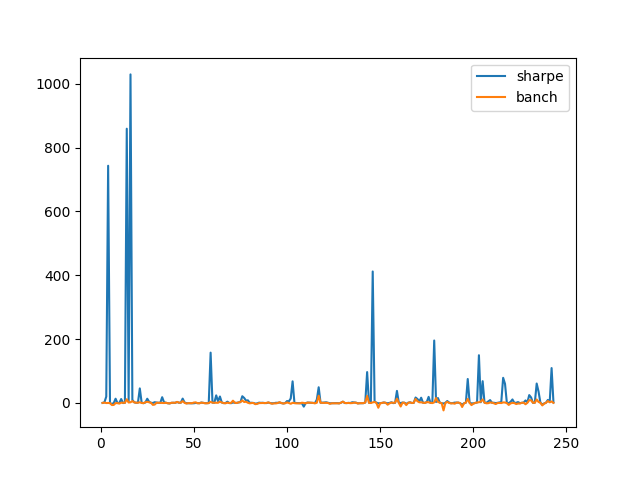
\includegraphics[clip, width=0.9\textwidth]{Graphics/trainPA00S.png} \caption{Sharpe Ratio of TRAIN 1}
\end{subfigure}%
\end{figure}

\newpage
\begin{figure}[H]
\begin{subfigure}{.5\textwidth}%
\centering
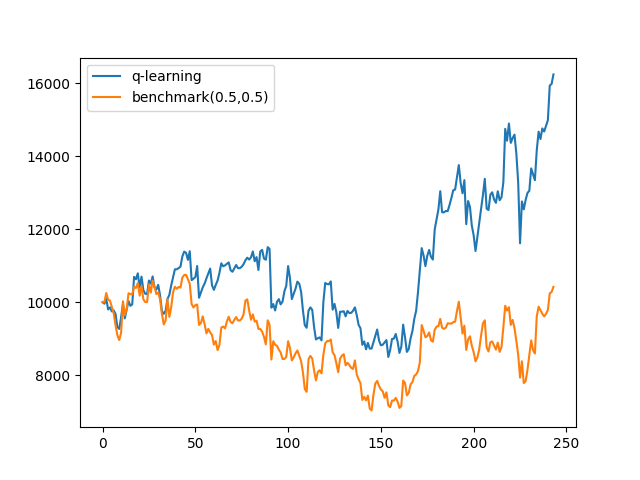
\includegraphics[clip, width=0.9\textwidth]{Graphics/trainPA33.png} \caption{TRAIN 4 (AMD \& MTN))} 
\end{subfigure}%
\begin{subfigure}{.5\textwidth}%
\centering
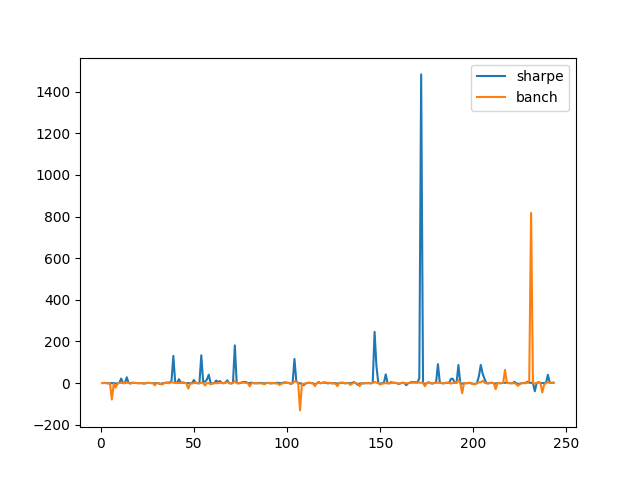
\includegraphics[clip, width=0.9\textwidth]{Graphics/trainPA33S.png} \caption{Sharpe Ratio of TRAIN 4}
\end{subfigure}%
\vspace{0.1cm}
\begin{subfigure}{.5\textwidth}%
\centering
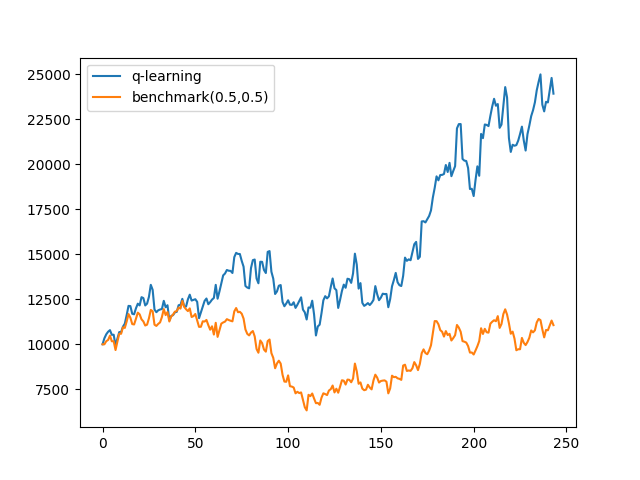
\includegraphics[clip, width=0.9\textwidth]{Graphics/trainPA99.png} \caption{TRAIN 9 (MU \& PPC))} 
\end{subfigure}%
\begin{subfigure}{.5\textwidth}%
\centering
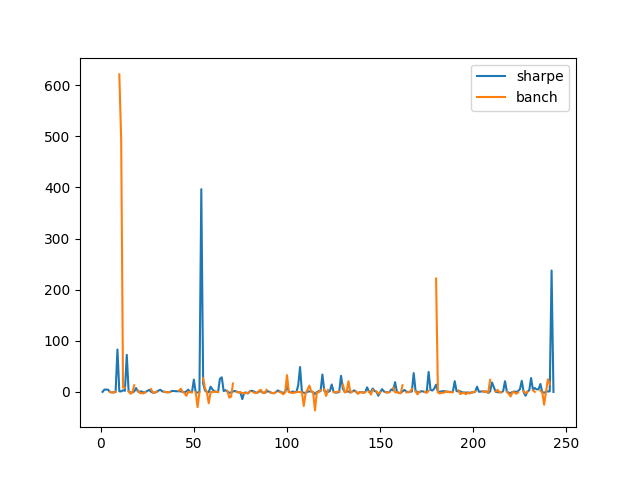
\includegraphics[clip, width=0.9\textwidth]{Graphics/trainPA99s.png} \caption{Sharpe Ratio of TRAIN 9}
\end{subfigure}%
\vspace{0.7cm}

Then we get the test result as follow:

\vspace{0.4cm}
\begin{subfigure}{.5\textwidth}%
\centering
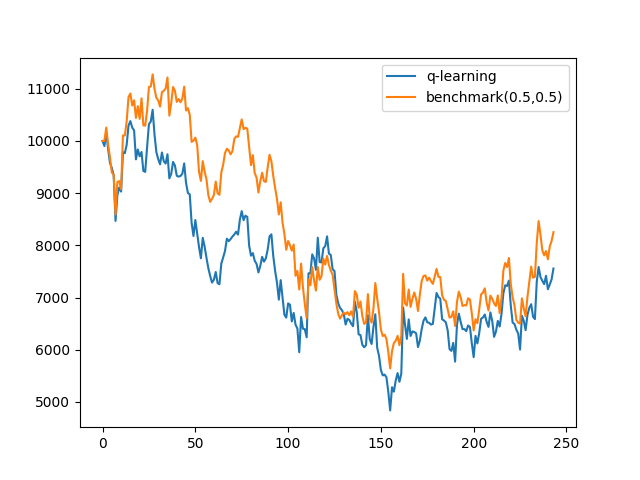
\includegraphics[clip, width=0.9\textwidth]{Graphics/TESTAC10.png} \caption{TEST 1 (AMAT \& CAJ)} 
\end{subfigure}%
\begin{subfigure}{.5\textwidth}%
\centering
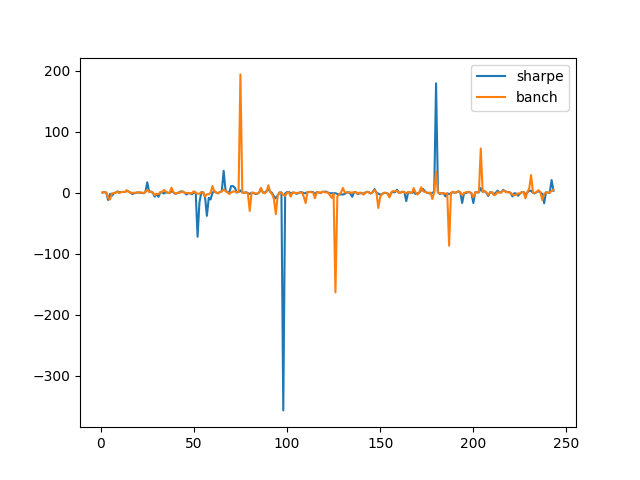
\includegraphics[clip, width=0.9\textwidth]{Graphics/TESTAC10S.png} \caption{Sharpe Ratio of TEST 1}
\end{subfigure}%
\end{figure}

\newpage
\begin{figure}[H]
\begin{subfigure}{.5\textwidth}%
\centering
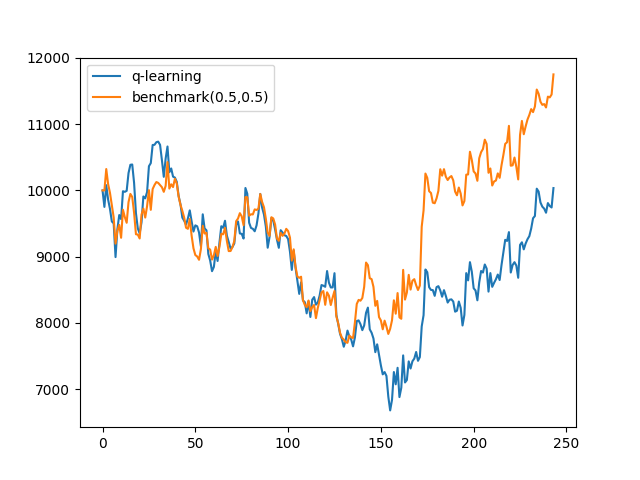
\includegraphics[clip, width=0.9\textwidth]{Graphics/TESTFC10.png} \caption{TEST 2 (FCX \& CAJ)} 
\end{subfigure}%
\begin{subfigure}{.5\textwidth}%
\centering
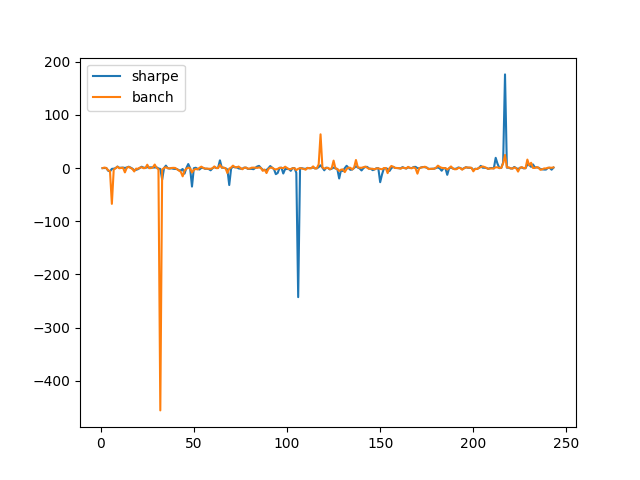
\includegraphics[clip, width=0.9\textwidth]{Graphics/TESTFC10S.png} \caption{Sharpe Ratio of TEST 2}
\end{subfigure}%
\vspace{0.4cm}

It is even worse than we use 3 days as a period.

\vspace{0.4cm}

However, if we use 3 days’ regression to test in the 10-day training q-table, we get the following testing result:

\vspace{0.4cm}

\begin{subfigure}{.5\textwidth}%
\centering
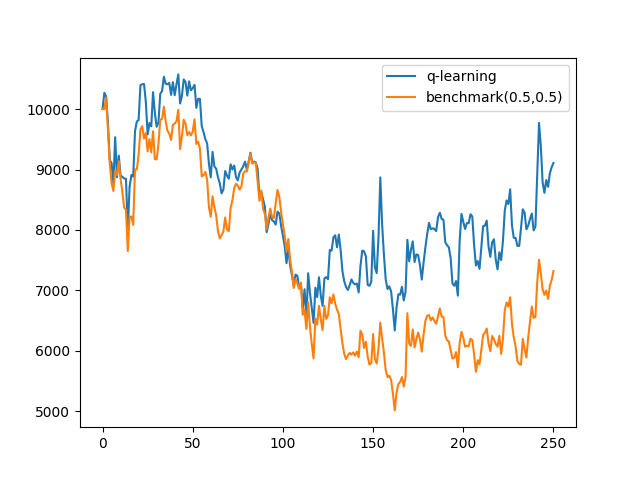
\includegraphics[clip, width=0.9\textwidth]{Graphics/TESTAC3Dby10train.png} \caption{TEST 1 (AMAT \& CAJ)} 
\end{subfigure}%
\begin{subfigure}{.5\textwidth}%
\centering
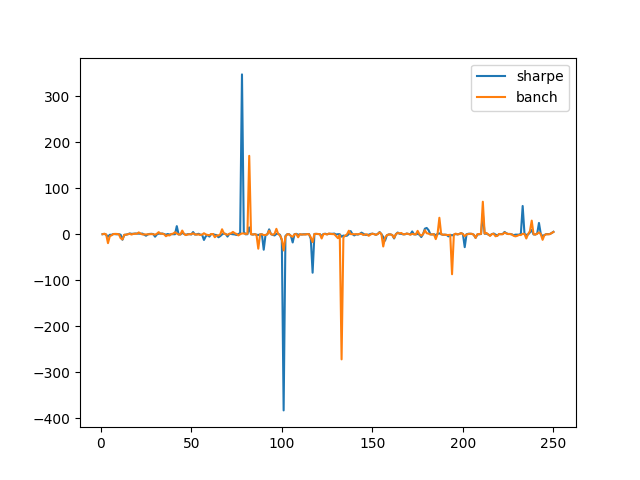
\includegraphics[clip, width=0.9\textwidth]{Graphics/TESTAC3Dby10trainS.png} \caption{Sharpe Ratio of TEST 1}
\end{subfigure}%
\vspace{0.4cm}
\begin{subfigure}{.5\textwidth}%
\centering
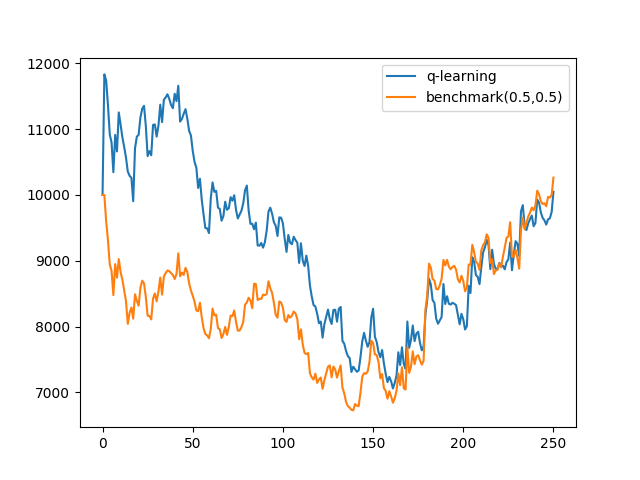
\includegraphics[clip, width=0.9\textwidth]{Graphics/TESTFC3Dby10train.png} \caption{TEST 1 (AMAT \& CAJ)} 
\end{subfigure}%
\begin{subfigure}{.5\textwidth}%
\centering
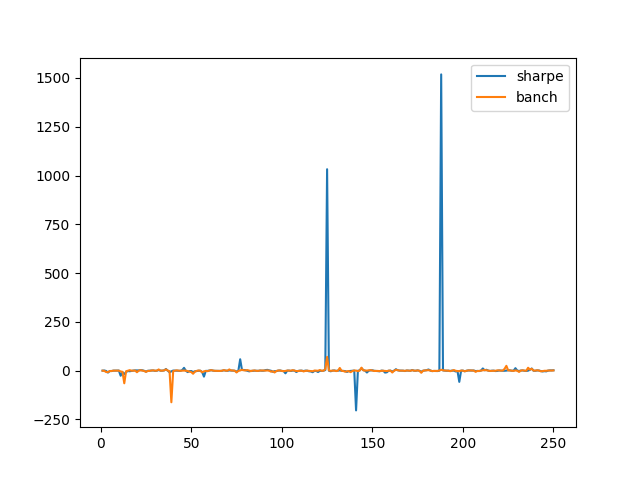
\includegraphics[clip, width=0.9\textwidth]{Graphics/TestFC3Dby10trainS.png} \caption{Sharpe Ratio of TEST 1}
\end{subfigure}%

\vspace{0.4cm}

It is better than both of using 10 days as a period to train and test and using 3 days as a period. Maybe training the model by using longer days as a period and test it by using shorter days as a period can get a better model.

\end{figure}

\newpage
\textbf{Using one pair of stocks’ 10 years data to train the model (n=3) using sharpe ratio as reward function}

We change the data we use. This time, we use the same one pair of stocks(AMAT \& CAJ) to train and test. We use 10 years data to train the model, and use the following one year of data to test it. And still use sharpe ratio as reward function.

\begin{figure}[H]
\begin{subfigure}{.5\textwidth}%
\centering
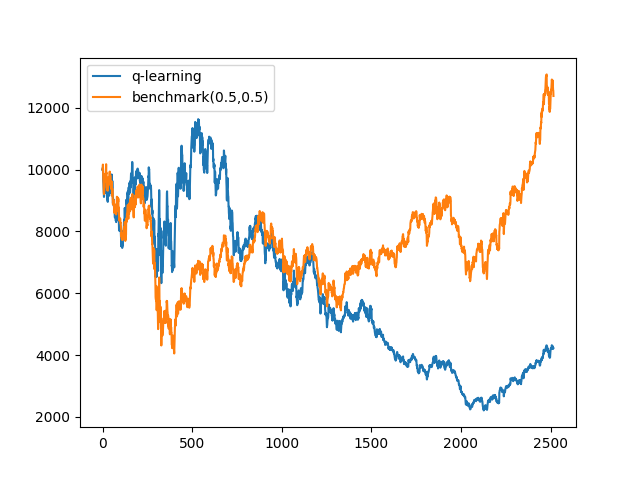
\includegraphics[clip, width=0.9\textwidth]{Graphics/NEW_TRY1.png} \caption{Training} 
\end{subfigure}%
\begin{subfigure}{.5\textwidth}%
\centering
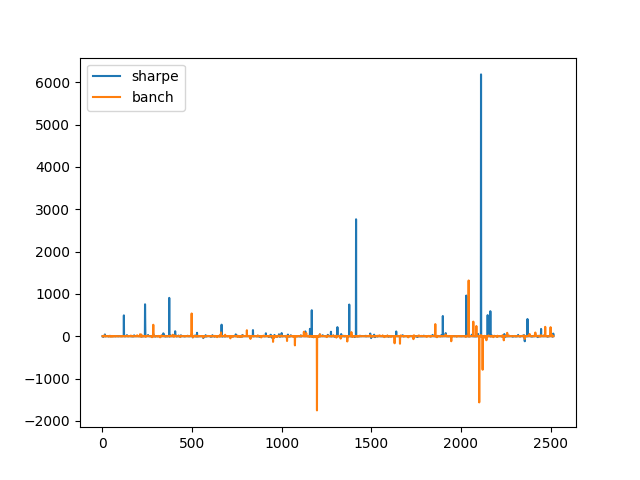
\includegraphics[clip, width=0.9\textwidth]{Graphics/NEW_TRY1S.png} \caption{Sharpe Ratio}
\end{subfigure}%
\vspace{0.4cm}
\begin{subfigure}{.5\textwidth}%
\centering
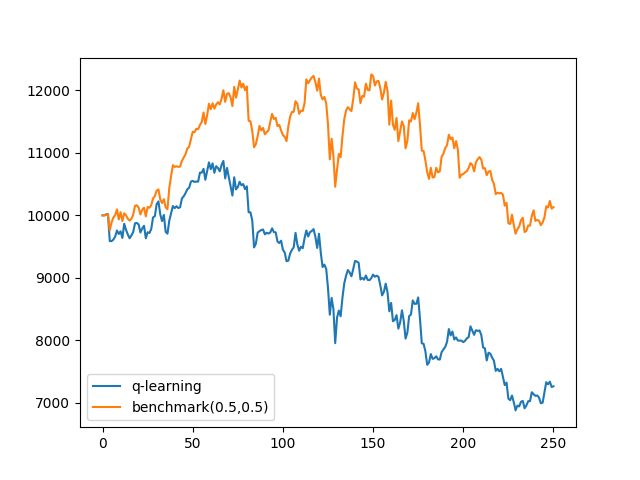
\includegraphics[clip, width=0.9\textwidth]{Graphics/NEW_TRY1TEST.png} \caption{Testing} 
\end{subfigure}%
\begin{subfigure}{.5\textwidth}%
\centering
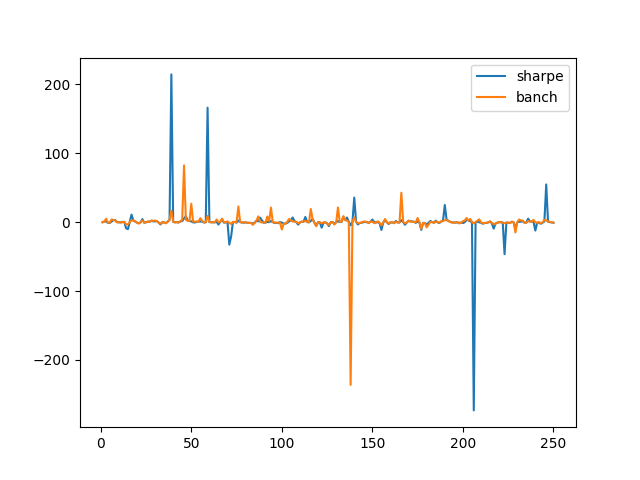
\includegraphics[clip, width=0.9\textwidth]{Graphics/NEW_TRY1TESTS.png} \caption{Sharpe Ratio}
\end{subfigure}%
\end{figure}

\newpage
Then we change to use total portfolio value as reward function
\begin{figure}[H]
\begin{subfigure}{.5\textwidth}%
\centering
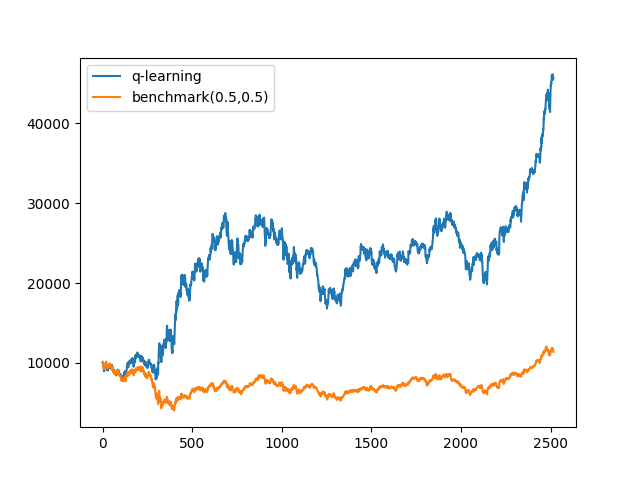
\includegraphics[clip, width=0.9\textwidth]{Graphics/New_try_rewardpv.png} \caption{Training} 
\end{subfigure}%
\begin{subfigure}{.5\textwidth}%
\centering
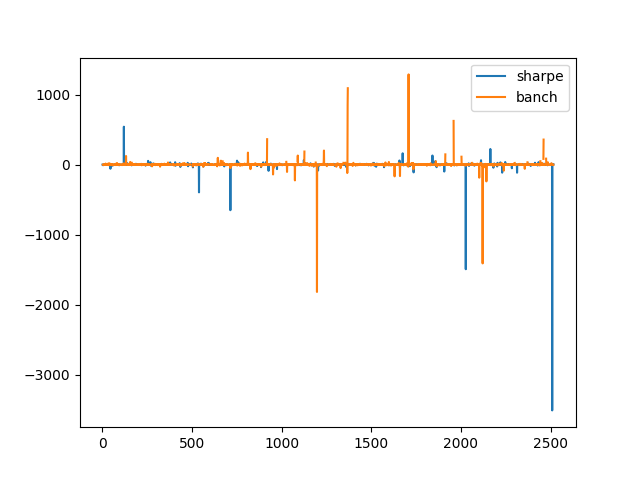
\includegraphics[clip, width=0.9\textwidth]{Graphics/new_try_rewardpvS.png} \caption{Sharpe Ratio}
\end{subfigure}%
\vspace{0.4cm}
\begin{subfigure}{.5\textwidth}%
\centering
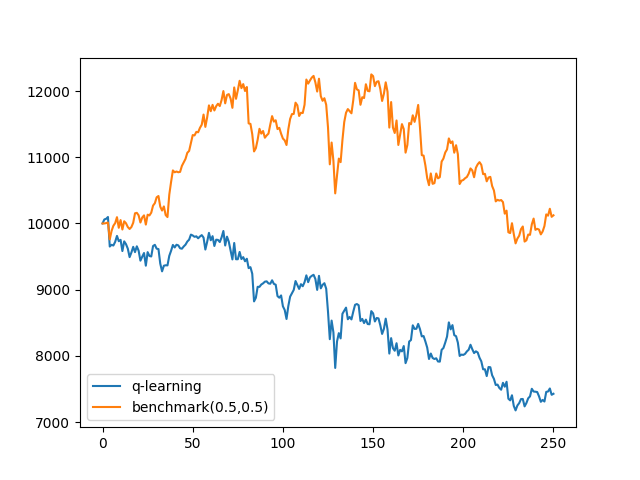
\includegraphics[clip, width=0.9\textwidth]{Graphics/NEW_TEST_REWARDPV.png} \caption{Testing} 
\end{subfigure}%
\begin{subfigure}{.5\textwidth}%
\centering
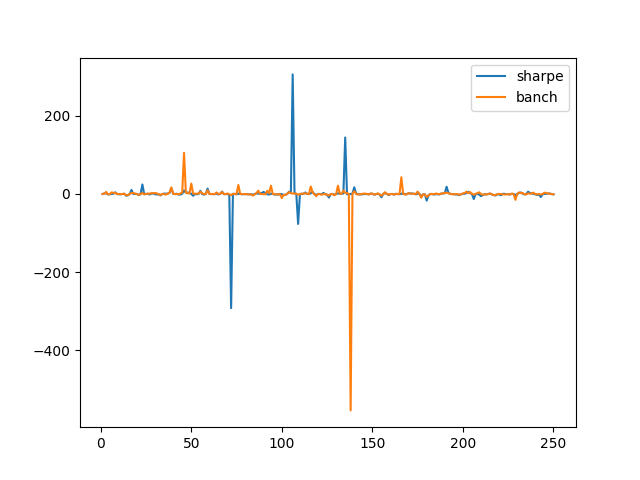
\includegraphics[clip, width=0.9\textwidth]{Graphics/REWARDPVS.png} \caption{Sharpe Ratio}
\end{subfigure}%
\end{figure}

\section{Deep Q-Network}

Q-learning has some obvious problems in our problem setting.
Firstly, to implement Q-learning we have to discretize the state, which is the stock price. However, if we discretize the stock price, the result we get will be inaccurate, which implies that the profit we get may not be optimized. Thus, it is necessary to find an alternative way that can handle the continuous state situation.

Secondly, it is impossible to find every Q-table value because there are tons of pairs of state and action in the project. Computer should be able to find action that fits our goal the most even when it runs into entirely new situation, but if Q-table values that computer finds are not enough computer will choose the action randomly. Thus, it is necessary to find another way that helps the computer find the right action without having to find out every single Q-table value directly.

To solve these two big problems, Deep Q Network is an appropriate method to solve them.

In our Deep Q Network algorithm, computer chooses action randomly with pre-determined probability, which is called ‘epsilon exploration’. It is mainly used in stochastic process like this situation where stock price changes randomly, because if without this epsilon exploration after one certain state happens computer choose the action depending on this specific state solely even though there are high probabilities the other states can happen as well. 
When neural networks are trained, we use mini-batch which picks items randomly in the memories which consists of plenty of pairs of state, action, reward, and next-state. In Q-learning, Q-table is updated with time and it is affected by time correlation. Unlike Q-learning, in Deep Q Network this algorithm called ‘Experience Replay’ is used to avoid correlation between each memory, especially with this kind of situation where time is related with, and it makes results better.     

In this project, fully connected layers, whose inputs are vectors, are used instead of convolutional neural networks, whose inputs are matrixes, because states in this project are price changes, which can be expressed more easily as vectors than matrixes. 

Relu and linear function are used as an activation function, Mean Squared Error function as a loss function, and Adam function as an optimizer. In terms of hyperparameters, we chose figures similar to those that are mainly used. 

\begin{figure}[H]
\begin{center}
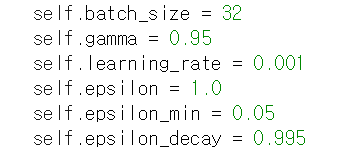
\includegraphics[clip, width=0.4\textwidth]{Graphics/image1.png} \caption{Hyperparameters}
\end{center}
\end{figure}

In this Deep Q network algorithm, only two stocks, Applied Materials Inc. (AMAT) and Canon Inc. (CAJ), are used through all procedures.

We do training and testing separately, 10-years data which is from 08/03/2007 to 08/02/2017 is used for training and 1-year data which is from 08/03/2017 to 08/02/2018 is used for testing.  

The state is a vector that has 58 elements, each of which is price change between the day before and the day of each stock, because we use 30-days stock price for both stock as the state. 

The action is categorized into 11 options, which is the ratio between two stocks from 0 : 1 to 1 : 0, changing by 0.1 each. 
Naturally in this way the reward becomes the profit made by changing the action after a day.

It implies that computer chooses the ratio between two stocks which maximizes the profit by considering stock price changes in 30 days. 
The starting budget is 10,000\$ and transaction fee is 0.2\% of total transaction amount as same as Q-Learning, and we train it for 3,000, 5,000, and 50,000 episodes, respectively.

The graph shows the price change of AMAT and CAJ for 10-years of training period which is from 08/03/2007 to 08/02/2017.
After 10 years, AMAT price increases to 1.97 times, and CAJ price decreases to 0.63 times. 

\begin{figure}[H]
\begin{center}
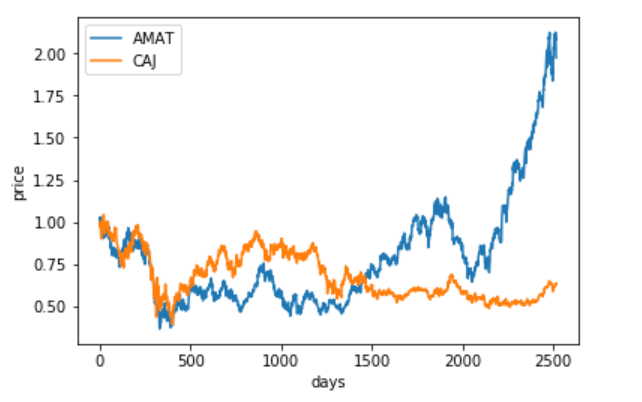
\includegraphics[clip, width=0.6\textwidth]{Graphics/image3.png} \caption{Data}
\end{center}
\end{figure}

\textbf{Training}

\begin{figure}[H]
\begin{center}
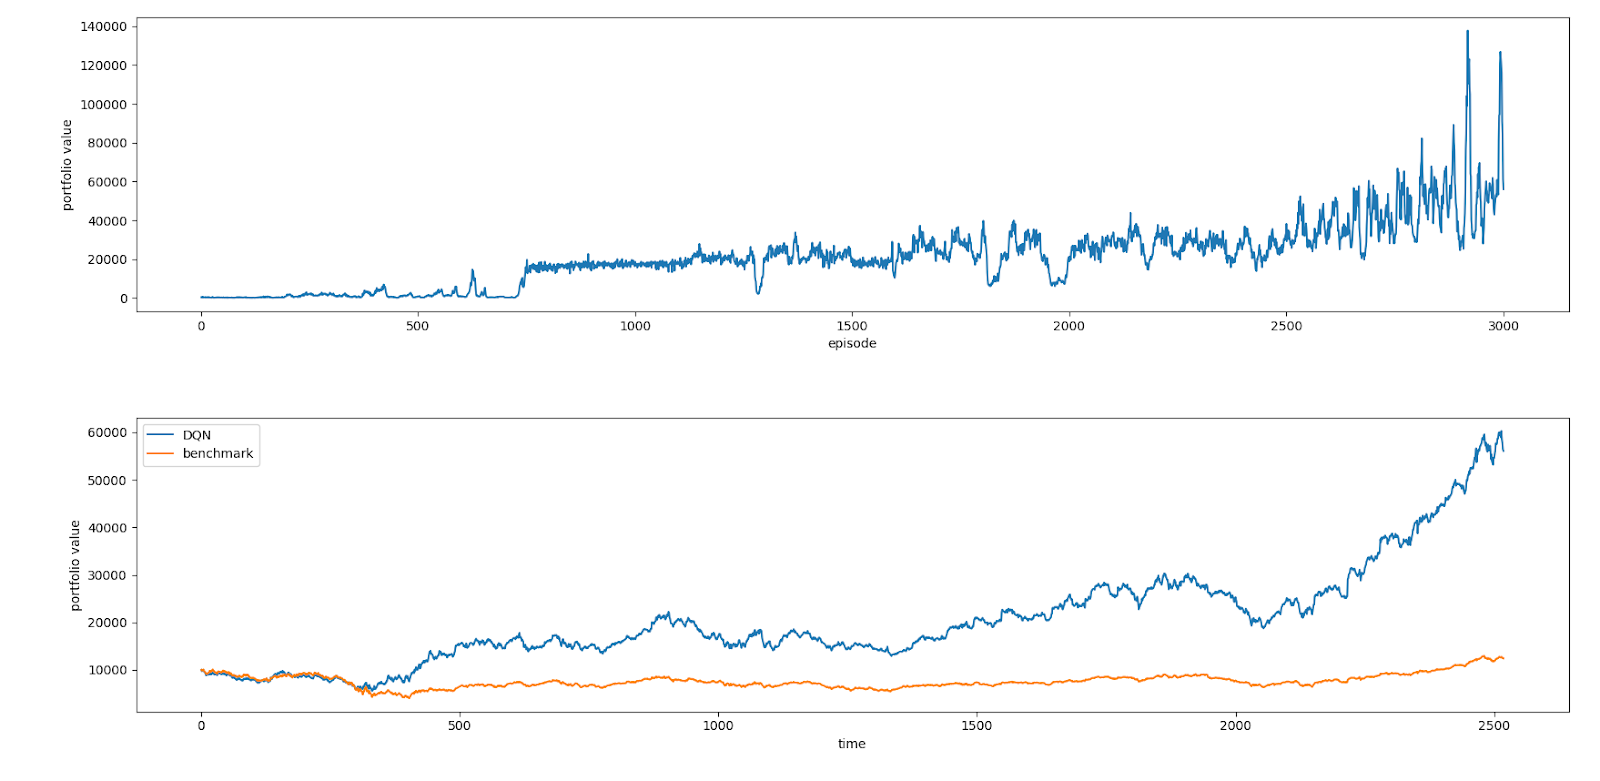
\includegraphics[clip, width=0.8\textwidth]{Graphics/image8.png} \caption{Training 1 : With 3,000 episodes }
\end{center}
\end{figure}

Upper graph shows that the portfolio value of the last day after 10 years of training for every episode. Due to 0.2\% transaction fee, from the beginning to around 700th episode, the portfolio value stays less than 1,000. It suddenly passes 10,000 at 747th episode, and keeps increasing and  fluctuating continuously until about 2,500th episode. From 2,500th episode, it starts to surge dramatically, and at 2,921th episode the portfolio value peaks at 123,074.  

Lower graph shows the portfolio value as day passes at the final episode, which is 3,000th. A benchmark is the strategy that we allocate half of total budget to each stock every day. The total portfolio value of the benchmark is 12,433. Even though the final episode that this graph shows is not the episode that makes the profit the most, we can easily notice from this graph that Deep Q Network works much better than the benchmark.  

Deep Q Network works well in training, but one weakness is that fluctuation of the portfolio value for every episode is too widely as upper graph shows. We changed figures of hyperparameters to solve this problem, but nothing was effective. 

One thing to take a notice from the upper graph is from around 2,500th episode, there is a trend that the portfolio value increases steadily. Thus, we decided to run the same code with 5000 episodes.

\begin{figure}[H]
\begin{center}
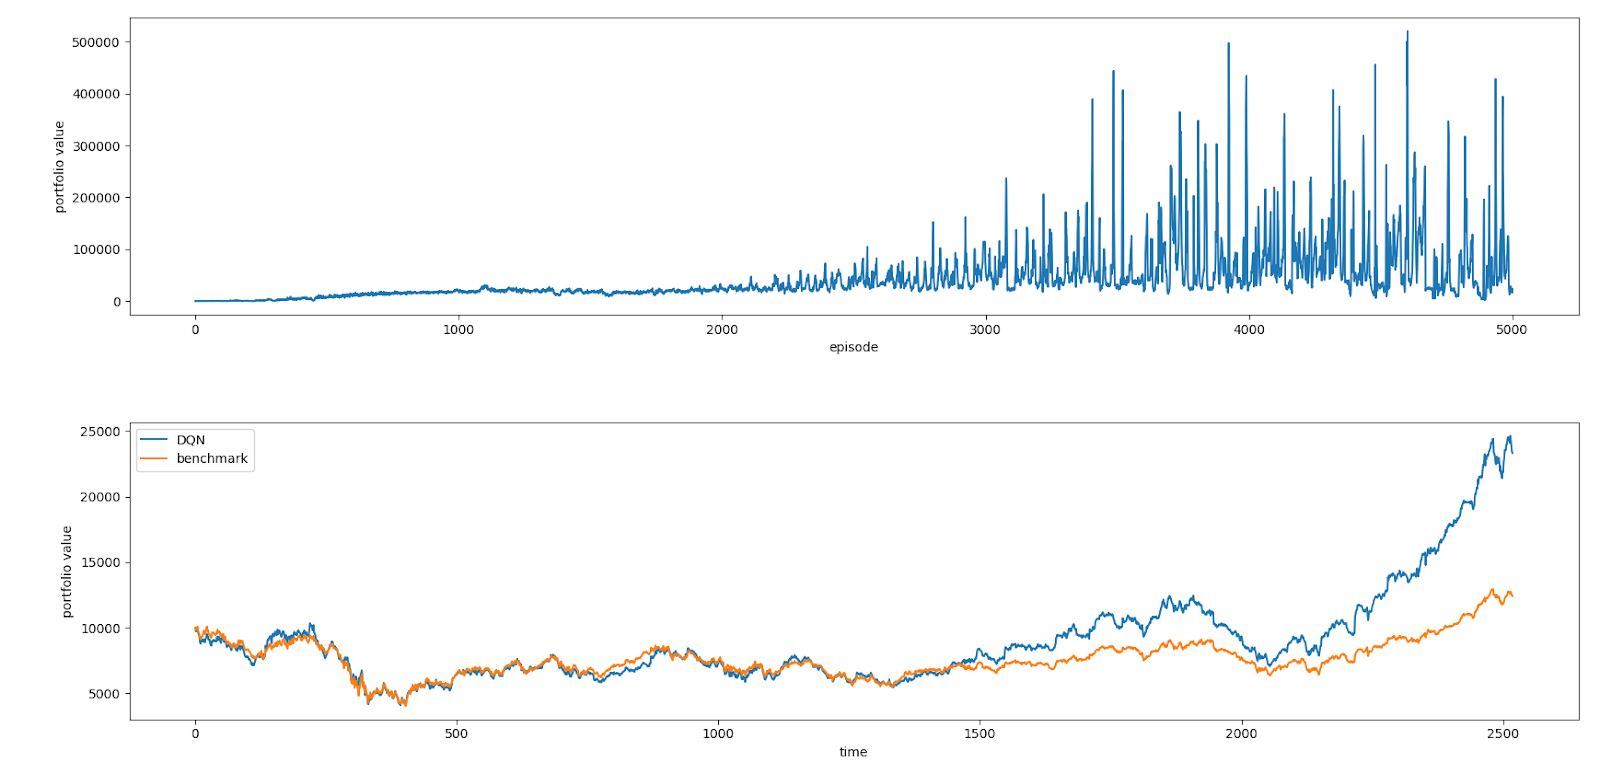
\includegraphics[clip, width=0.8\textwidth]{Graphics/image10.png} \caption{Training 2 : With 5,000 episodes }
\end{center}
\end{figure}

As we guessed, in upper graph, after 3000th episode there are much more peaks than before. The maximum portfolio value is 520,438 with 4,602th episode. 

However, the weakness Deep Q Network has, fluctuating too much, was not solved at all. In the graph below, the result of 5000th episode is even worse, ending with only 23,321 portfolio value, comparing to 4,602th episode which ends with 520,438 portfolio value. 

Thus, hoping that it could be solved if the number of episodes increases a lot, thus we increased the number of episodes to 50,000.

\begin{figure}[H]
\begin{center}
\includegraphics[clip, width=0.8\textwidth]{Graphics/image9.png} \caption{Training 3 : With 50,000 episodes }
\end{center}
\end{figure}

The portfolio value of the last day still varies too much for every episode, but maximum portfolio value increased again. The maximum portfolio value is 914,586 which happened at 37,042th episode. It seems that a trend that maximum portfolio value increases as an episode goes stops, so we decided to stop training.  

Overall, training takes about 53 seconds per 100 episodes on average.

\begin{figure}[H]
\begin{center}
\includegraphics[clip, width=0.6\textwidth]{Graphics/image4.png} \caption{Data}
\end{center}
\end{figure}

For 1-year testing period, average of the prices of these two stocks do not change much, and after one year the average is almost same as the start point. 

We picked a model which has maximum portfolio value from each of three results. Thus, for 3,000 episodes, we picked 2,921th episode which has 123,074 portfolio value, for 5,000 episodes, we picked 4,602th episode which has 520,438 portfolio value, and for 50,000 episodes, we picked 37,042th episode which has 914,586 portfolio value. 

The benchmark is same with training, each stock has half of total budget for every single day.

\begin{figure}[H]
\begin{center}
\includegraphics[clip, width=0.6\textwidth]{Graphics/image6.png} \caption{Testing (3,000 episodes)}
\end{center}
\end{figure}

\begin{figure}[H]
\begin{center}
\includegraphics[clip, width=0.6\textwidth]{Graphics/image5.png} \caption{Testing (5,000 episodes)}
\end{center}
\end{figure}

\begin{figure}[H]
\begin{center}
\includegraphics[clip, width=0.6\textwidth]{Graphics/image7.png} \caption{Testing (50,000 episodes)}
\end{center}
\end{figure}

The portfolio value on the last day of a benchmark is 10,217, whereas the portfolio value for testing with the best result among 3,000 episodes is 9,217, a portfolio value for testing with the best result among 5,000 episodes is 6,511, and a portfolio value for testing with the best result among 5,000 episodes is 8,401. 

The point of these observation is that how good the result for training is has no relationship with how good the result for testing. Moreover, all three results have less portfolio value than the benchmark which just keeps the ratio with 50:50 for every single day. 

The chart below summarizes our results for both training and testing by Deep Q-Network. 

\begin{figure}[H]
\begin{center}
\includegraphics[clip, width=0.6\textwidth]{Graphics/image2.png} \caption{Comparasion}
\end{center}
\end{figure}
\subsection{Including Exchange Ratio}
In the later state of the project, we try to include the exchange ratio into our consideration. The application is that you can include two different countries' stock into the portfolio and settle at the end of the date with one of the stocks' currency in the portfolio. Since sometime due to the difference of public holiday and time-zone in different countries, we may face the situation that one country's stock market is working while the other one is not. When we face such situation, we will just skip that date in our training model.

The way we calculate the portfolio value is as follows
$$ pv_{t} = pv_{t-1} *[ (p_{t} / p_{t-1}) * w_{1}  + (q_{t} / q_{t-1}) * w_{2} * cv_{t}/cv_{t-1})]$$
the portfolio value will be in the currency you have chosen.
\endinput


